\documentclass[letterpaper,10pt]{article}

\usepackage[utf8]{inputenc}
\usepackage{tocloft}                        %Modify table of contents (toc)      
\renewcommand{\contentsname}{\hfill\bfseries\Large Contents\hfill}   %center toc title
\renewcommand{\cftaftertoctitle}{\hfill}
\renewcommand{\cftsecleader}{\cftdotfill{\cftdotsep}}   %put .... in toc
\usepackage{rotating}
\usepackage{url}                            %put websites in paper
\usepackage[margin=0.8in]{geometry}         %adjust margins
\usepackage{graphicx}                       %use images
\graphicspath{ {./Figures/} } %where to find files
\usepackage[outdir=./Figures/]{epstopdf}
\usepackage{sectsty}                        %center section titles
%\allsectionsfont{\centering}
\usepackage{chngcntr}                       %Start Figure counting according to section
\counterwithin{figure}{section}             %where to start that counter
\usepackage[section]{placeins}              %able to use Floatbarrier
\usepackage{caption}
\usepackage{subcaption}                     %subfigures allowed
\usepackage{amsmath}                        %math stuff
\usepackage{verbatim}                        %block commenting
\usepackage{color} 
\renewcommand{\thefootnote}{\fnsymbol{footnote}} % modify footnotes to symbols

\begin{document}

\title{Electromagnetic Calorimeter System Operations Manual}

\vskip 0.5cm

\author{L.C Smith, Jefferson Laboratory\\[0.2ex]
{\it ec\_manual.tex -- v1.1}}

\date \today
%
\maketitle

\begin{abstract}
This document provides an overview of the CLAS12 Electromagnetic Calorimeter (EC) System and serves 
as an Operations Manual for the detector. Instructions are provided for shift workers related to 
basic steps of operating and monitoring the HV controls, monitoring the detector system and 
responding to alarms, and knowing when to contact the on-call personnel. More complete details 
are also provided for EC system experts regarding the channel mapping to the readout electronics, 
the cable connections and routing in Hall~B, higher-order high voltage system operations, and 
detector servicing. This document also provides references to the available EC documentation and 
a list of personnel authorized to perform EC system repairs and modify system settings.
\end{abstract}

\thispagestyle{empty}

\clearpage

\vfil
\eject

\tableofcontents

\vfil
\eject

\section{EC Overview}
\label{intro}

The CLAS12 EC package includes the legacy CLAS6 electromagnetic calorimeters (ECAL) and new pre-shower
calorimeter (PCAL) modules installed just upstream of ECAL.  Six sectors of EC in CLAS12 will be used
primarily for identification of electrons, photons (including $\pi^0\rightarrow 2\gamma$ decays), and
neutrons.
Both PCAL and ECAL are triangular-shaped sampling calorimeters. The calorimeter design uses
a lead-scintillator sandwich consisting of alternating layers of 1-cm thick scintillators and ~2 mm thick
lead sheets. At 11 GeV the total thickness corresponds to about 21 radiation lengths. Scintillator layers
are grouped into three stereo views, called U, V, and W,  which are readout using photomultiplier tubes (PMT).
Specifications for each calorimeter are outlined below. 

%%%%%%%%%%%%%%%%%%%%%%%%%%%%%%%%%%%%%%%%%%%%%%%%%%%%%%%%%%%%%%%%%%%%%%%%%%%%%%%%%%%%%%%%%%%%%%%%%%%%%
\begin{figure}[htbp]
  \centering
  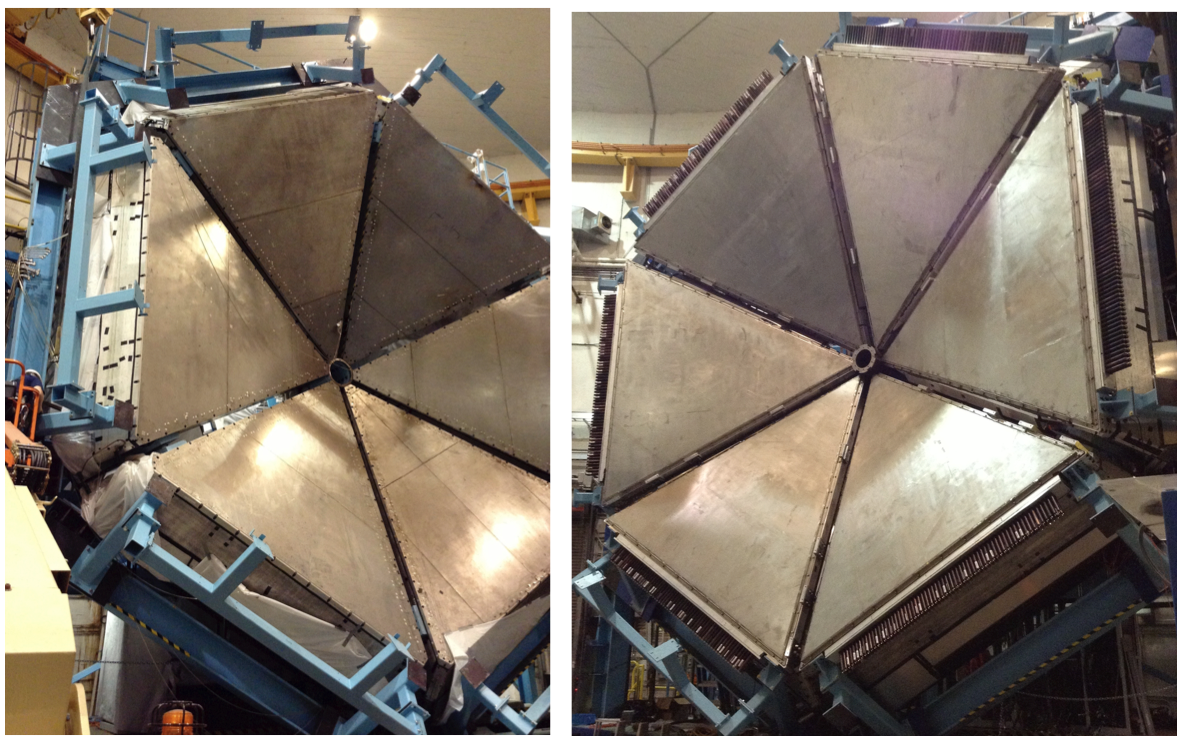
\includegraphics[width= 5in, keepaspectratio = true]{fc-pcal-ecal}
  \vspace{2mm}
\caption{Photographs of the ECAL (left) and PCAL (right) calorimeter modules installed on the Forward
    Carriage in Hall B.  The Forward Carriage is roughly 10~m in diameter.}
  \label{fwd_car}
\end{figure}
%%%%%%%%%%%%%%%%%%%%%%%%%%%%%%%%%%%%%%%%%%%%%%%%%%%%%%%%%%%%%%%%%%%%%%%%%%%%%%%%%%%%%%%%%%%%%%%%%%%%%


%%%%%%%%%%%%%%%%%%%%%%%%%%%%%%%%%%%%%%%%%%%%%%%%%%%%%%%%%%%%%%%%%%%%%%%%%%%%%%%%%%%%%%%%%%%%%%%%%%%%%
\begin{table}[htbp]
\begin{center}
\begin{tabular}{|l|l|} \hline
{\bf Parameter}        & {\bf Design Value} \\ \hline \hline
{\bf PCAL}         &              \\ \hline 
Calorimeter type   & Sampling, lead-scintillator \\ \hline
Number of modules  & 6  \\ \hline
Module shape and dimensions & Triangle, base 394.3 cm height 385.3 cm \\ \hline
Total coverage area      &  45 m$^2$ \\ \hline
Distance from Target & 7.0 m \\ \hline
Angular coverage   & $\theta$: 5$^\circ$ $\to$ 35$^\circ$,$\phi$: 50\% at 5$^\circ$ $\to$ 85\% at 35$^\circ$ \\ \hline
Lead sheets & 2.2 mm thick (two pieces) \\ \hline
Number of scintillator layers & 15 per module \\ \hline
Number of lead sheets  & 14 per module \\ \hline
Number of stereo readout views & 3 (5 scintillator layers per view) \\ \hline
Scintillator material & Extruded polystyrene w/ 2 fiber holes\\ \hline
Scintillator core & Dow Styron 663 W \\ \hline
Scintillator cladding & Polystyrene with 12$\%$ TiO2 (0.25 mm) \\ \hline
Scintillator strip dimensions & 1 x 4.5 x 2.5-394(U)432(V,W) cm \\ \hline
Scintillator readout & WLS fibers (Kuraray Y-11 1mm DC) \\ \hline
Scintillators/module & U:84 V:77 W:77 \\ \hline
Scintillators readout/module & U:68 V:62 W:62 \\ \hline
Number of WLS fibers & 4 fibers/strip 1428/module \\ \hline
Number of readout channels & 192 per module \\ \hline
Readout PMT & Hamamatsu R6095 \\ \hline
Light yield & 11-12 photo e-/MeV \\ \hline 
\end{tabular}
\end{center}
\caption{PCAL technical design parameters.} 
\end{table}
\begin{table}[htbp]
\begin{center}
\begin{tabular}{|l|l|} \hline
{\bf Parameter}        & {\bf Design Value} \\ \hline \hline
{\bf ECAL}         &              \\ \hline
Calorimeter type   & Sampling, lead-scintillator \\ \hline
Number of modules  & 6 (each module has inner/outer segmentation and readout)\\ \hline
Module shape and dimensions & Triangle, base 420 cm height 388.8 cm \\ \hline
Total Coverage Area      & 49 m$^2$ \\ \hline
Distance from Target & 7.5 m (target center to upstream face) \\ \hline
Angular Coverage   & $\theta$: 5$^\circ$ $\to$ 35$^\circ$,$\phi$: 50\% at 5$^\circ$ $\to$ 85\% at 35$^\circ$ \\ \hline
Lead sheets & 2.387 mm thick (single piece)\\ \hline
Number of scintillator layers & 39 per module (15 inner, 24 outer) \\ \hline
Number of lead sheets  & 38 per module \\ \hline
Number of stereo readout views & 3 (5/8 scintillator layers per view for inner/outer) \\ \hline
Scintillator material & BC-412\\ \hline
Scintillator cladding & None. Teflon film (0.00762 cm) between layers. \\ \hline
Scintillator strip dimensions & 1 x 10.0 x 15-420 cm \\ \hline
Scintillator readout & BCF98 3mm cladded optical fiber \\ \hline
Scintillators/module & U:36 V:36 W:36 \\ \hline
Number of fibers & 22 fibers per PMT, 110/176 per inner/outer view \\ \hline
Number of readout channels & 216 per module \\ \hline
Readout PMTs & Phillips XP2262 and EMI 9954 \\ \hline
Light yield & 3-4 photo e-/MeV \\ \hline \hline
{\bf Expected Performance} & {\bf Value} \\ \hline
Energy resolution & 10$\%/\sqrt E$ (ECAL+PCAL) \\ \hline
Position resolution & 0.5 cm \\ \hline
Time resolution & 500 ps \\ \hline

\end{tabular}
\end{center}
\caption{ECAL technical design parameters.} 
\label{tab:ftofproperties}
\end{table}

\newpage

A block diagram of the readout electronics for the EC system is shown in 
Figure~\ref{readout-elec}. Signal cables are routed from the PMT locations on the calorimeter
modules to UVA 122B splitter panels located on the front of the electronics racks. The cable
connections are BNC at the PMT anode and LEMO at the splitter.  From the splitter, patch cables
are routed to VME DSC2 leading edge discriminators (for pulse timing measurements) and JLAB 250~MHz VME Flash
ADCs (FADC250) (for pulse amplitude measurements.)  The TDCs are CAEN VME 1190A with 100~ps LSB resolution.
The FADC250 and DSC2/TDC modules are housed in separate VXS crates.  The FADC250/VXS crate contains the
Virtual Trigger Processor (VTP) in a special switched slot which will be used to process energy and hit data for
trigger decision making.

%%%%%%%%%%%%%%%%%%%%%%%%%%%%%%%%%%%%%%%%%%%%%%%%%%%%%%%%%%%%%%%%%%%%%%%%%%%%%%%%%%%%%%%%%%%%%%%%%%%%%
\begin{figure}[htbp]
  \centering
  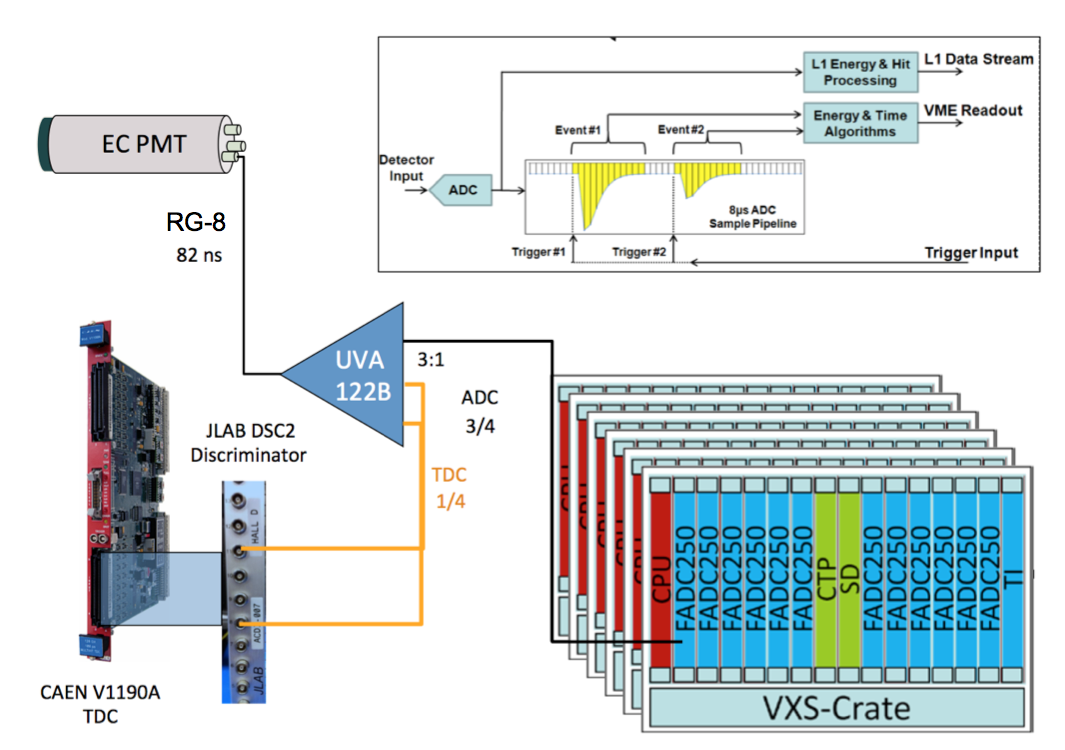
\includegraphics[width= 7in, keepaspectratio = true]{readout-electronics}
  \vspace{2mm}
  \caption{Schematic of signal readout electronics for ECAL system.  Shown are the cable and split ratios for the ECAL
    PMTs.  The PCAL case is similar but uses different split ratios.  Not shown are HV connections.  For ECAL transition patch cables were used at either end of the RG-8 signal cable, which are not shown here.
  }
  \label{readout-elec} 
\end{figure}
%%%%%%%%%%%%%%%%%%%%%%%%%%%%%%%%%%%%%%%%%%%%%%%%%%%%%%%%%%%%%%%%%%%%%%%%%%%%%%%%%%%%%%%%%%%%%%%%%%%%%

The electronics for each sector are located behind the detectors on the three levels of the Forward 
Carriage as follows:

\vskip 0.5cm

\begin{minipage}{0.5\textwidth}
\begin{itemize}
\item EC S1: FC Level 2 South (Beam left)
\item EC S2: FC Level 3 South (Beam left)
\item EC S3: FC Level 3 North (Beam right)
\end{itemize}
\end{minipage}
\begin{minipage}{0.5\textwidth}
\begin{itemize}
\item EC S4: FC Level 2 North (Beam right)
\item EC S5: FC Level 1 North (Beam right)
\item EC S6: FC Level 1 South (Beam left)
\end{itemize}
\end{minipage}

\vskip 0.5cm

Note that ``South'' refers to beam left and ``North'' to beam right (closer to the Pie Tower).

Figure~\ref{fc-layout-1} shows the Forward Carriage rack locations for the ECAL VME electronics and signal cable patch 
panels.  Note the rack layout for beam left is a mirror image of the layout for beam right.  Also the Level 1 rack layout
is different due to an alternate cable routing (discussed later).  A photograph of the Sector 6 rack installation is
shown in Figure~\ref{fc-layout-2}.

The HV power supplies for all PMTs in each ECAL sector are either CAEN 1527LC mainframes or CAEN 4527 mainframes 
outfitted with negative polarity 24-channel A1535N cards which fit into slots at the rear of each
mainframe. The HV mainframes that power the PCAL 
system are actually shared between the FTOF and the PCAL. The FTOF boards occupy slots 0 to 7 of each 
mainframe and the PCAL boards occupy slots 8 to 15 of each mainframe. These supplies are named HVFTOFn, 
n=1$\to$6 (i.e. HVFTOF1 $\to$ HVFTOF 6). The HV mainframes for the EC modules are named HVECALn (n=1$\to$6).
Figure~\ref{fc-layout-1} shows the locations of the HV mainframes for each of the EC sectors on the Forward Carriage.


%%%%%%%%%%%%%%%%%%%%%%%%%%%%%%%%%%%%%%%%%%%%%%%%%%%%%%%%%%%%%%%%%%%%%%%%%%%%%%%%%%%%%%%%%%%%%%%%%%%%%
\begin{figure}[htbp]
  \centering
  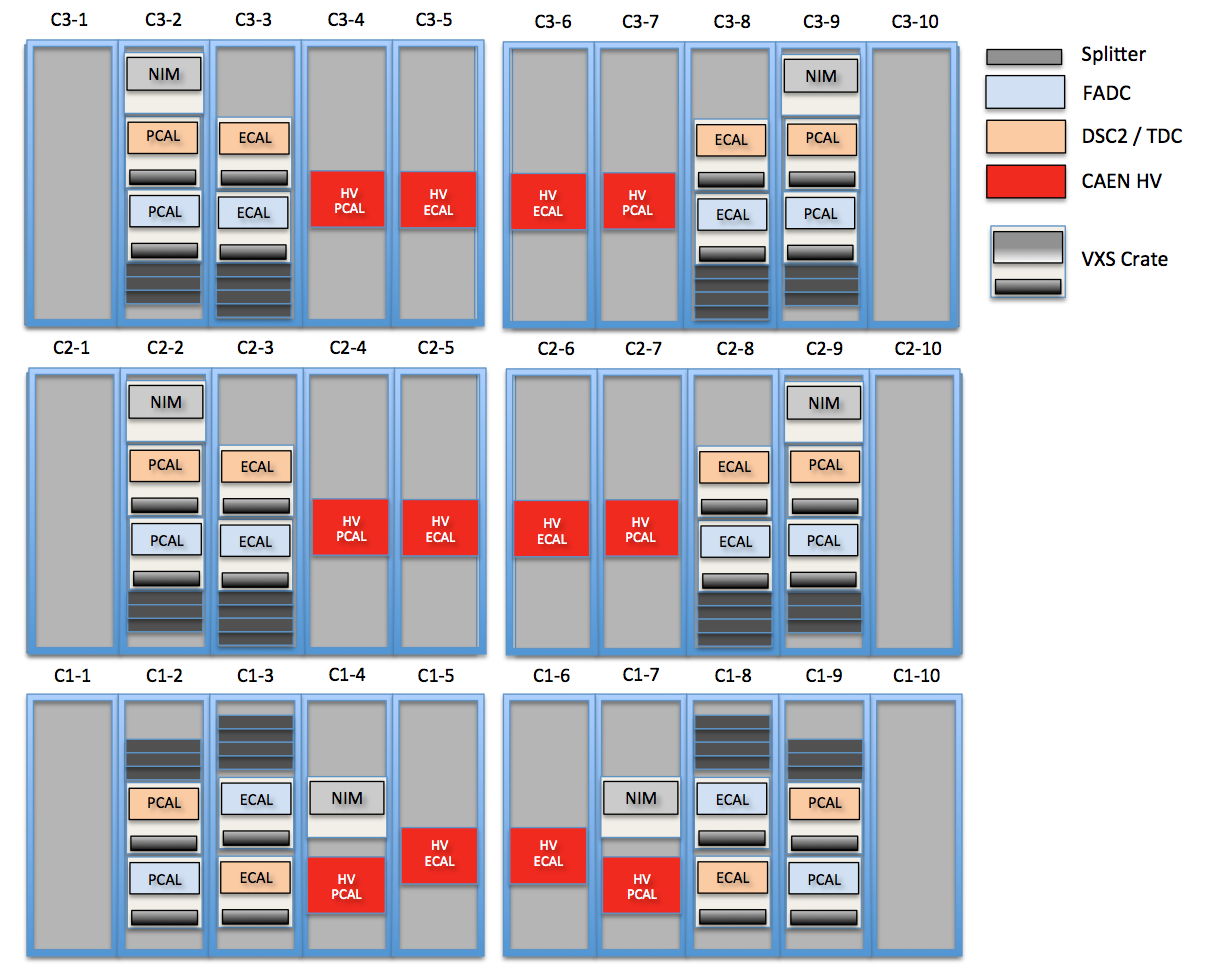
\includegraphics[width= 7in, keepaspectratio = true]{FC-EC-rack-layout-2}
  \vspace{2mm}
  \caption{Schematic layout of the EC VME electronics, signal cable splitters, and HV power 
  supplies in the electronics racks on each of the three levels of the Forward Carriage. The rack names on each level (c1, c2,
  and c3) are numbered 1 through 10.}
  \label{fc-layout-1} 
\end{figure}
%%%%%%%%%%%%%%%%%%%%%%%%%%%%%%%%%%%%%%%%%%%%%%%%%%%%%%%%%%%%%%%%%%%%%%%%%%%%%%%%%%%%%%%%%%%%%%%%%%%%%

%%%%%%%%%%%%%%%%%%%%%%%%%%%%%%%%%%%%%%%%%%%%%%%%%%%%%%%%%%%%%%%%%%%%%%%%%%%%%%%%%%%%%%%%%%%%%%%%%%%%%
\begin{figure}[htbp]
  \centering
  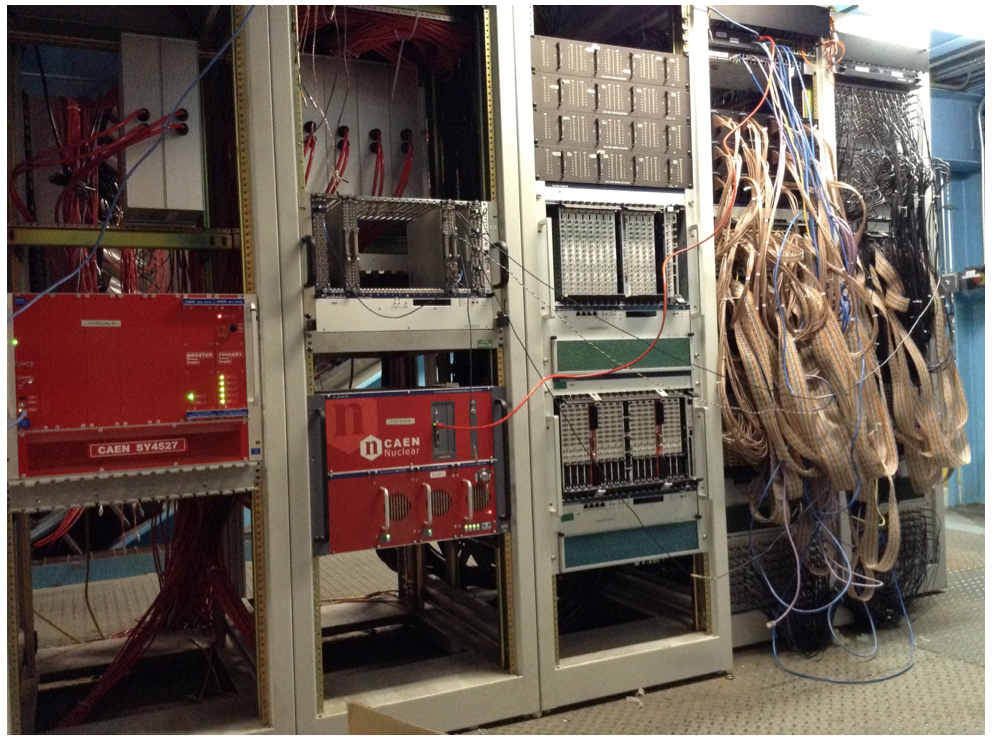
\includegraphics[width= 5in, keepaspectratio = true]{Sector6-electronics}
  \vspace{2mm}
  \caption{Photograph of racks C1-6 through C1-10 (Sector 6) during cable installation.  The rack with
    no cables installed (C1-8) houses four ECAL splitter panels (top), the FADC250 VXS crate (middle)
    and DSC2/TDC VXS crate (bottom).  The CAEN HV mainframe $\it{hvecal6}$ is at far left in rack C1-6,
    and the PCAL/FTOF mainframe $\it{hvftof6}$ is to the right in rack C1-7.}
  \label{fc-layout-2} 
\end{figure}
%%%%%%%%%%%%%%%%%%%%%%%%%%%%%%%%%%%%%%%%%%%%%%%%%%%%%%%%%%%%%%%%%%%%%%%%%%%%%%%%%%%%%%%%%%%%%%%%%%%%%


\clearpage

\vfil
\eject


\section{Information for Shift Workers}

\subsection{Shift Worker Responsibilities}

The shift worker in the Hall~B Counting House has five responsibilities with regard to the EC
system:

\begin{enumerate}
\item Updating the Hall~B electronic logbook with records of problems or system conditions (see 
Section~\ref{logbook}).

\item Contacting EC system on-called personnel for any problems that are discovered (see 
Section~\ref{contact}).

\item Responding to EC system alarms from the Hall~B alarm handler (see Section~\ref{alarms}).

\item Turning on or off the high voltage for the EC system using the HV control interface (see 
Section~\ref{hv-control}).

\item Monitoring the hit occupancy scalers for the system (see Section~\ref{monitoring}).
\end{enumerate}

\subsubsection{Updating the Logbook}
\label{logbook}

The electronic logbook (or e-log)~\cite{e-log} is set up to run on a specified terminal in the 
Hall~B Counting House. Shift workers are responsible for keeping an up-to-date and accurate record
of any problems or issues concerning the EC system. For any questions regarding the logbook, its
usage, or on what is considered to be a ``logbook worthy'' entry, consult the assigned shift leader.

Note the shift worker should follow all posted or communicated instructions about entering ECAL
scaler screens into the e-log. This is typically done once per 8-hour shift as directed on the
shift checklist.

\subsubsection{Contacting EC System Personnel}
\label{contact}

As a general rule, shift workers should spend no more than 10 to 15 minutes attempting to solve
any problem that arises with the EC system. At that point they should contact the assigned 
EC on-call worker to either provide advice on how to proceed or to address the problem.

This document is divided into a section for shift workers and EC system experts. However, only 
EC system experts (as listed in Section~\ref{personnel}) are authorized to make changes to the EC
parameter settings, to work on the hardware or electronics, or to modify the DAQ system 
software. This division between shift worker responsibilities and expert responsibilities is
essential to maintain in order to protect and safeguard the equipment, to ensure data collection
is as efficient as possible, and to minimize down time. If the shift worker has any question 
regarding how to proceed when an issue arises, the shift leader should be consulted.

\subsubsection{Hall~B Alarm Handler}
\label{alarms}

The BEAST alarm handler system running in the Counting House monitors the entire Hall~B Slow Controls
system. This include HV and LV systems, gas systems, torus and solenoid controls, subsystem
environment controls (e.g. temperature, humidity), and pulser calibration systems (among several
others). The system runs on a dedicated terminal in the Counting House. One of the main responsibilities
of the shift worker is to respond to alarms from this system, either by taking corrective action
or contacting the appropriate on-call personnel. Instructions and details on the alarm handler for Hall~B
are given in Ref.~\cite{beast}.

For the EC system, the only element of the system monitored by the alarm handler is the HV system.
Whenever any PMT HV either trips off or changes beyond a pre-determined window an alarm will sound.
The alarm handler will identify the specific channel (or channels) causing the alarm. These channels can
be reset either through the alarm handler or through the nominal EC HV control screens. These channels
should be reset only after identifying the cause of the alarm.  Beam-current related trips can be reset
immediately once beam conditions have stabilized.  Instability in the HV due to a malfunction in the PMT,
HV divider or HV power supply should be diagnosed and noted in the e-log so repairs can be made at
the next Hall entry.  

\subsection{High Voltage Controls}
\label{hv-control}

Control of the EC HV mainframes is through the Hall~B CS-Studio suite, which is an Eclipse-based collection 
of tools used as an interface to the EPICS Slow Control system. To start the user interface on any 
terminal in the Hall~B Counting House, enter the command {\it clascss}. Figure~\ref{ecal-screen} 
shows the control panel that is launched.
%%%%%%%%%%%%%%%%%%%%%%%%%%%%%%%%%%%%%%%%%%%%%%%%%%%%%%%%%%%%%%%%%%%%%%%%%%%%%%%%%%%%%%%%%%%%%%%%%%%%%
\begin{figure}[htbp]
  \centering
  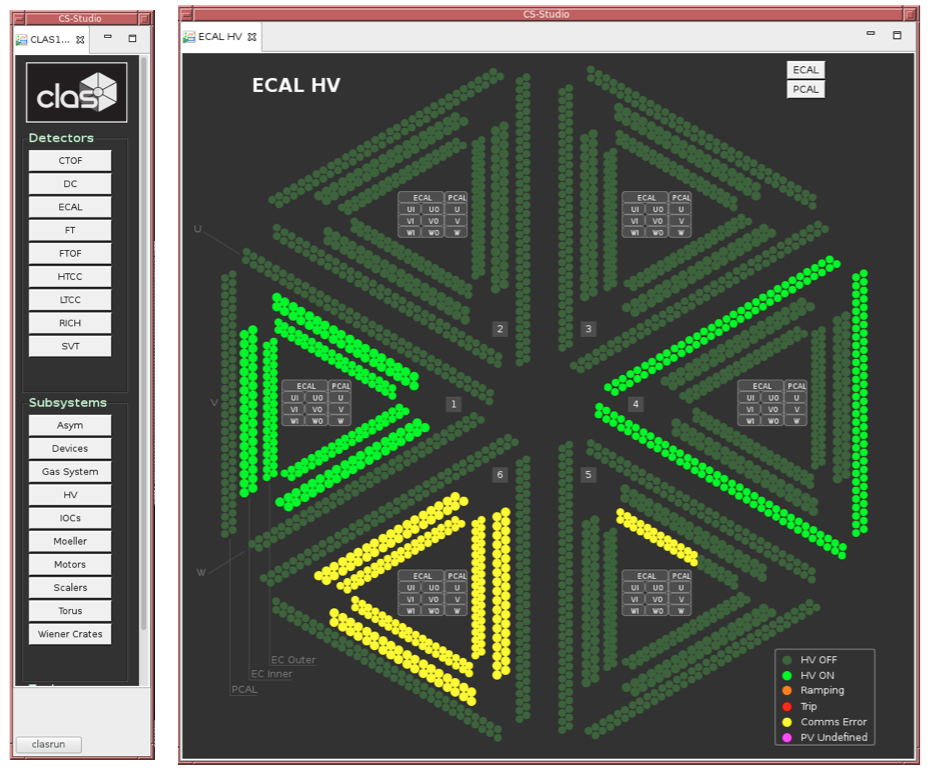
\includegraphics[width= 6in, keepaspectratio = true]{cssclas-detector-interface}
  \vspace{2mm}
  \caption{Left: The CS-Studio interface used for the Slow Controls of the CLAS12 detectors and subsystems.  ECAL HV
    controls may be accessed through either the ``ECAL'' button under Detectors or the ``HV'' button under Subsystems.
  Right: Detector based ECAL HV display and control interface. For each sector the outermost triangle represents the PCAL, while
  ECinner and ECouter are the middle and innermost triangles respectively. Individual PMT HV channel controls
  are indicated by small circles. HV channel status is indicated by the colormap at lower right.  An entire sector
  of PMTs (EC+PCAL) may be turned on and off by clicking the sector number at the apex of the triangle.}
  \label{ecal-screen}
\end{figure}
%%%%%%%%%%%%%%%%%%%%%%%%%%%%%%%%%%%%%%%%%%%%%%%%%%%%%%%%%%%%%%%%%%%%%%%%%%%%%%%%%%%%%%%%%%%%%%%%%%%%%

HV controls are presented in two ways: either mapped to the physical detector (sector,layer,component) or
mapped to the HV mainframe (crate,slot,channel).
To access detector-based EC HV controls, click on the ``ECAL'' button on the Detectors list. This pops up a 
sub-menu of all Slow Controls subprograms for the ECAL system.  Clicking on ``EC HV''
will bring up the HV control panel shown in Figure~\ref{ecal-screen} (right). This interface allows
simple ON/OFF HV operations which are detailed in Figure~\ref{ecal-screen2}.

For the shift worker the most common operations are turning off and on large groups of PMTs.  These
group operations are accessed via the pop-up menus which appear when clicking on the labels shown in
Figure~\ref{ecal-screen2} and described below:

\begin{enumerate}
\item Turning on and off all PMTs within a single sector.
\item Turning on and off all PMTs within a single calorimeter (ECAL or PCAL).
\item Turning on and off all PMTs within a single U,V,W view of a single calorimeter.
\end{enumerate}

In addition to group ON/OFF operations it may be occasionally necessary to access single PMTs in order to
enable, disable, change the HV or alter various set-points for that specific PMT.  This is accomplished by
either clicking on the ``Controls'' selection in Figure~\ref{ecal-screen2} which brings up all PMTs corresponding
to a (U,V,W) view, or clicking on the circular icon corresponding to the desired PMT (see Figure~\ref{ecal-screen3})
to bring up just the panel for that PMT.
%%%%%%%%%%%%%%%%%%%%%%%%%%%%%%%%%%%%%%%%%%%%%%%%%%%%%%%%%%%%%%%%%%%%%%%%%%%%%%%%%%%%%%%%%%%%%%%%%%%%
\begin{figure}[htbp]
  \centering
  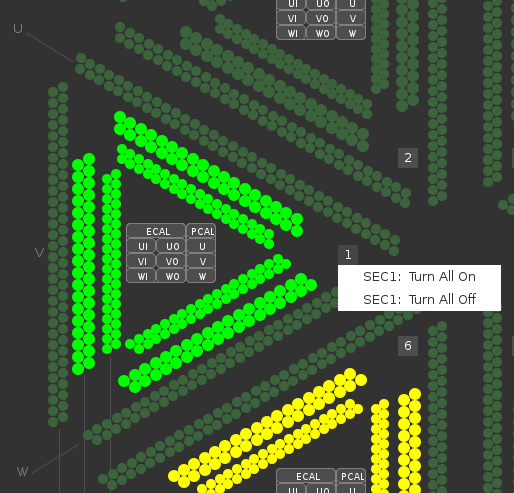
\includegraphics[width= 5in, keepaspectratio = true]{ecal-hv-screen-5}
  \vspace{2mm}
  \caption{Detail of Fig.~\ref{ecal-screen} which shows sector ``1''
    has been selected, activating the pop-up option menu.  Individual controls for modules are
    labeled ``ECAL'', ``PCAL'' and for individual views ``U,V,W'' which provide similar pop-up menus
    as shown.  Control of individual PMTs within a view is possible by clicking the circular elements.  }
  \label{ecal-screen2}
\end{figure}
%%%%%%%%%%%%%%%%%%%%%%%%%%%%%%%%%%%%%%%%%%%%%%%%%%%%%%%%%%%%%%%%%%%%%%%%%%%%%%%%%%%%%%%%%%%%%%%%%%%%%
%%%%%%%%%%%%%%%%%%%%%%%%%%%%%%%%%%%%%%%%%%%%%%%%%%%%%%%%%%%%%%%%%%%%%%%%%%%%%%%%%%%%%%%%%%%%%%%%%%%%%
\begin{figure}[htbp]
  \centering
  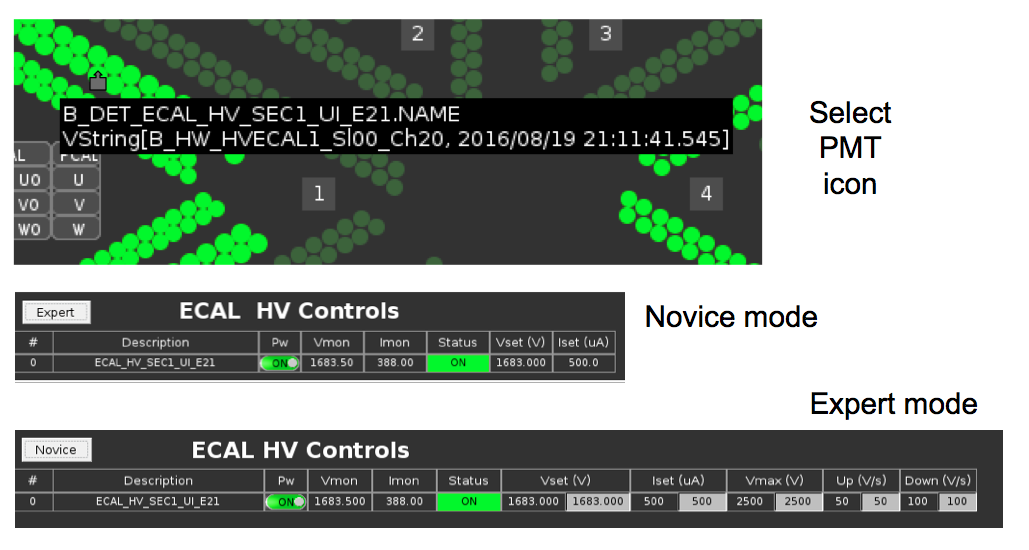
\includegraphics[width= 6in, keepaspectratio = true]{expert-novice}
  \vspace{2mm}
  \caption{ECAL HV displays for single PMT HV controls.  Hover the mouse over the PMT icons to
    view popup of EPICS Property Value (PV) identifier. Select the desired PMT to bring up Novice
    mode controls (middle) which allow only OFF/ON control via the Pw button.  Click Expert button to
    bring up controls for voltage (Vset), maximum HV divider current (Iset), maximum HV (Vmax), HV ramp
  rates (Up,Down). Note these settings apply only to the PMT selected, not all PMTs.}
  \label{ecal-screen3}
\end{figure}
%%%%%%%%%%%%%%%%%%%%%%%%%%%%%%%%%%%%%%%%%%%%%%%%%%%%%%%%%%%%%%%%%%%%%%%%%%%%%%%%%%%%%%%%%%%%%%%%%%%%%

If a single PMT is selected, a window similar to Fig.~\ref{ecal-screen3} (middle) is displayed. This
window shows the monitored channel voltage and currennt $V_{mon}$ (V) and $I_{set}$ ($\mu$A), the channel status (OFF, ON),
and the demand or set channel voltage $V_{set}$ (V).  Also shown is the maximum permissible HV divider
current $I_{set}$ ($\mu$A).  This interface would be used by shift workers to enable or disable a
PMT via the Pw button.

In the upper left corner of the window is a button marked ``Expert'' that
brings up the window shown at the botton of Fig.~\ref{ecal-screen3}. This window allows changes to the system settings
for the maximum channel current, maximum channel voltage setting, and the channel HV ramp up and 
ramp down rates.   Clicking on the ``Novice'' button
in the upper left corner toggles between the 
expert and novice screens. \textcolor{red}{The expert screen should only be used by the list of 
authorized EC personnel given in Section~\ref{personnel}.} 

The HV Control Interface screen (see Fig.~\ref{ecal-screen}) also provides a color key to indicate 
the channel status:

\begin{itemize}
\item HV off - no highlight color (channel color dark green)
\item HV on - bright green
\item HV ramping up or ramping down - orange
\item HV trip - red
\item Communication problem - yellow
\item Undefined channel status - magenta
\end{itemize}

When HV controls are unresponsive or HV monitoring stripcharts appear to become static it is likely
to be an EPICS communication error due to an IOC process that cannot communicate with the hardware or a
server.  Sometimes the hardware is at fault and has to be rebooted or power-cycled.  Usually this
requires an IOC reboot.  Controls for monitoring IOC status and rebooting frozen IOCs are available from
several menus.  For the EC HV system the IOC screen can be reached from the CSS menu via the ``HV''
button under Subsystems (see Figure~\ref{ecal-screen4}.)  To reboot the
IOC for a specific mainframe, click on the ``Restart iocHV*'' button corresponding to the desired mainframe.
PMT channels for which an IOC reboot is necessary will illuminate yellow as illustrated for the EC Sector 6 PMTs
in Figure~\ref{ecal-screen}.

%%%%%%%%%%%%%%%%%%%%%%%%%%%%%%%%%%%%%%%%%%%%%%%%%%%%%%%%%%%%%%%%%%%%%%%%%%%%%%%%%%%%%%%%%%%%%%%%%%%%%
\begin{figure}[htbp]
  \centering
  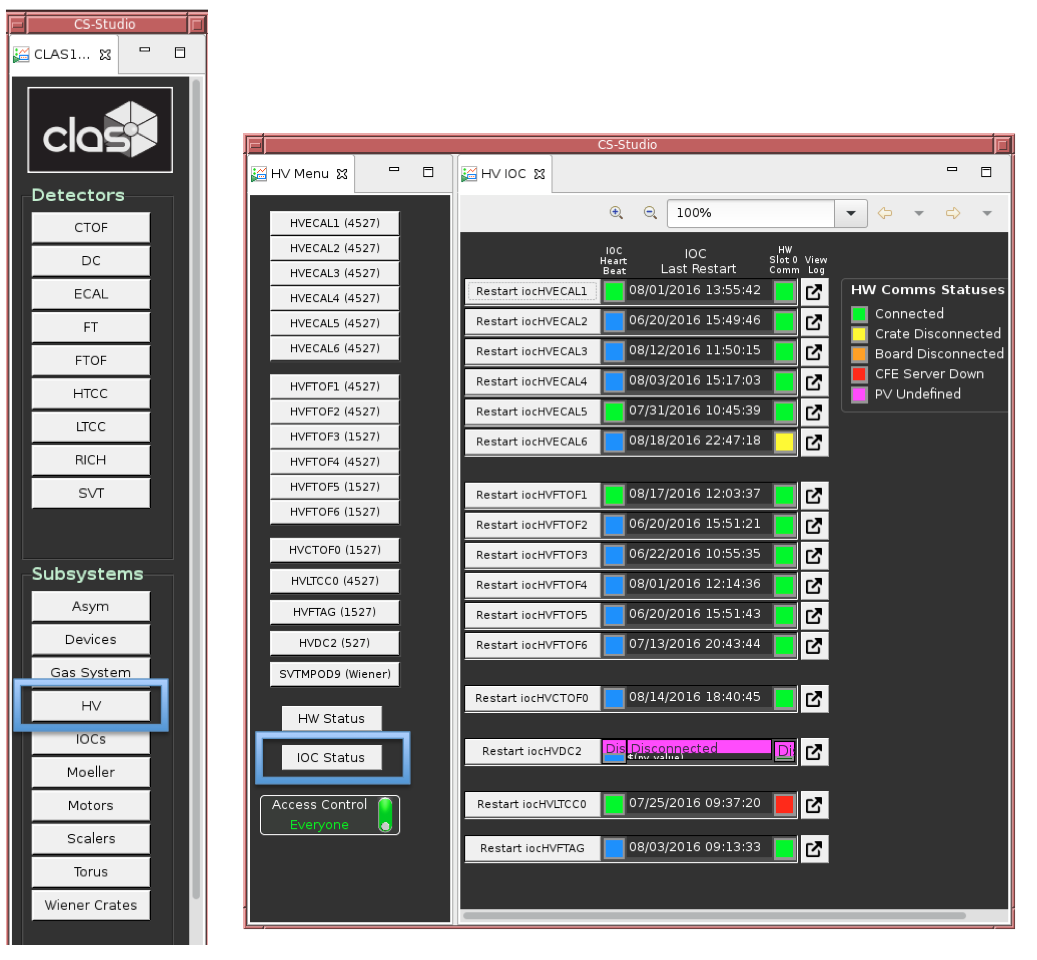
\includegraphics[width= 6in, keepaspectratio = true]{HV_IOC_2}
  \vspace{2mm}
  \caption{EPICS IOC status and controls are available from the CSS Main Menu by clicking on ``HV'' under ``Subsystems'',
    then clicking on ``IOC Status''.  This will be necessary whenever HV Mainframes are power-cycled or otherwise
  interrupted, or if the HW Comms Status lights are anything but green, or the IOC ``HeartBeat'' is not blinking green.}
  \label{ecal-screen4}
\end{figure}
%%%%%%%%%%%%%%%%%%%%%%%%%%%%%%%%%%%%%%%%%%%%%%%%%%%%%%%%%%%%%%%%%%%%%%%%%%%%%%%%%%%%%%%%%%%%%%%%%%%%%

\vfil
\eject

\subsection{Detector Monitoring}
\label{monitoring}

A number of monitoring tools to study the performance of the Forward Carriage detector systems
have been prepared. A hierarchy of tools is desirable to allow quick access to detector status
without the necessity of bringing up the Data Acquistion (DAQ).  One of the earliest tools developed
was a ROOT-based GUI called FCMON~\cite{fcmon} to monitor and display scalers for the
Forward Carriage detectors.  To launch this program from any Counting House computer, type {\it fcmon}.
This brings up the window as shown in Figure~\ref{fcmon1} (left). This tool enables display of
the scalers from all forward carriage discriminators and FADCs for each of the six CLAS12 sectors. To
use the interface for EC, click on the sector of interest in the left column, click on ECAL or PCAL in
the center column, and then click on the source of the scalers in the third column. To bring
up the scaler display screens, select ``Scalers'' under the ``Monitor'' drop down menu as
shown in Figure~\ref{fcmon1} (right).
 
%%%%%%%%%%%%%%%%%%%%%%%%%%%%%%%%%%%%%%%%%%%%%%%%%%%%%%%%%%%%%%%%%%%%%%%%%%%%%%%%%%%%%%%%%%%%%%%%%%%%%
\begin{figure}[htbp]
  \centering
  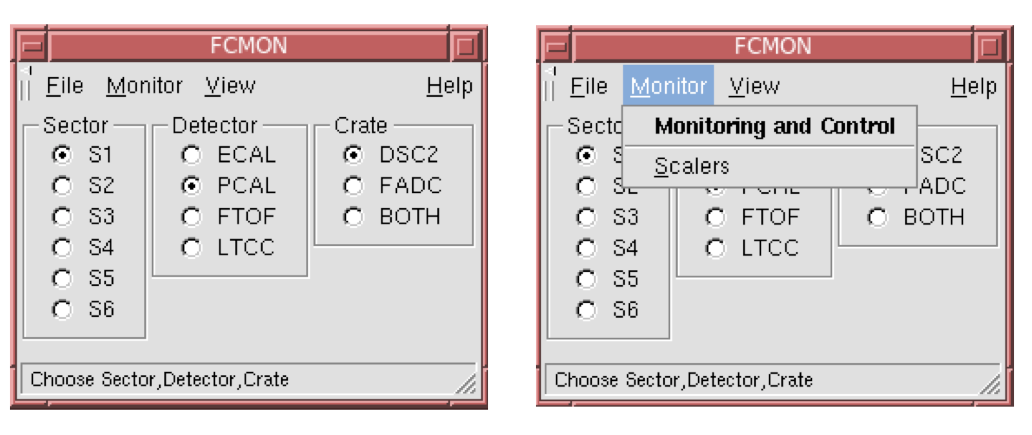
\includegraphics[width= 6in, keepaspectratio = true]{fcmon-1}
  \vspace{2mm}
  \caption{Forward Carriage scaler display program {\it fcmon}. (Left) Main screen. (Right) Menu selection to
    access scaler display window.  Click on ``scalers''.}
\label{fcmon1}
\end{figure}
%%%%%%%%%%%%%%%%%%%%%%%%%%%%%%%%%%%%%%%%%%%%%%%%%%%%%%%%%%%%%%%%%%%%%%%%%%%%%%%%%%%%%%%%%%%%%%%%%%%%%

The EC scalers can be monitored in one of three different ways by selecting the appropriate tab
at the top of the scaler display screen (see Fig.~\ref{fcmon2}). These three modes include:

\begin{itemize}
\item Slots: Scaler rate values (Hz) displayed for each VXS crate slot,channel housing the DSC2 or FADC modules.
\item Rates: Scaler rate values (Hz) plotted for each physical EC detector channel.
\item Stripcharts: Scaler rate values (Hz) plotted as a 2D strip chart (rate (z) vs. counter (y)  vs. time (x))
\end{itemize}

%%%%%%%%%%%%%%%%%%%%%%%%%%%%%%%%%%%%%%%%%%%%%%%%%%%%%%%%%%%%%%%%%%%%%%%%%%%%%%%%%%%%%%%%%%%%%%%%%%%%%
\begin{figure}[htbp]
  \centering
  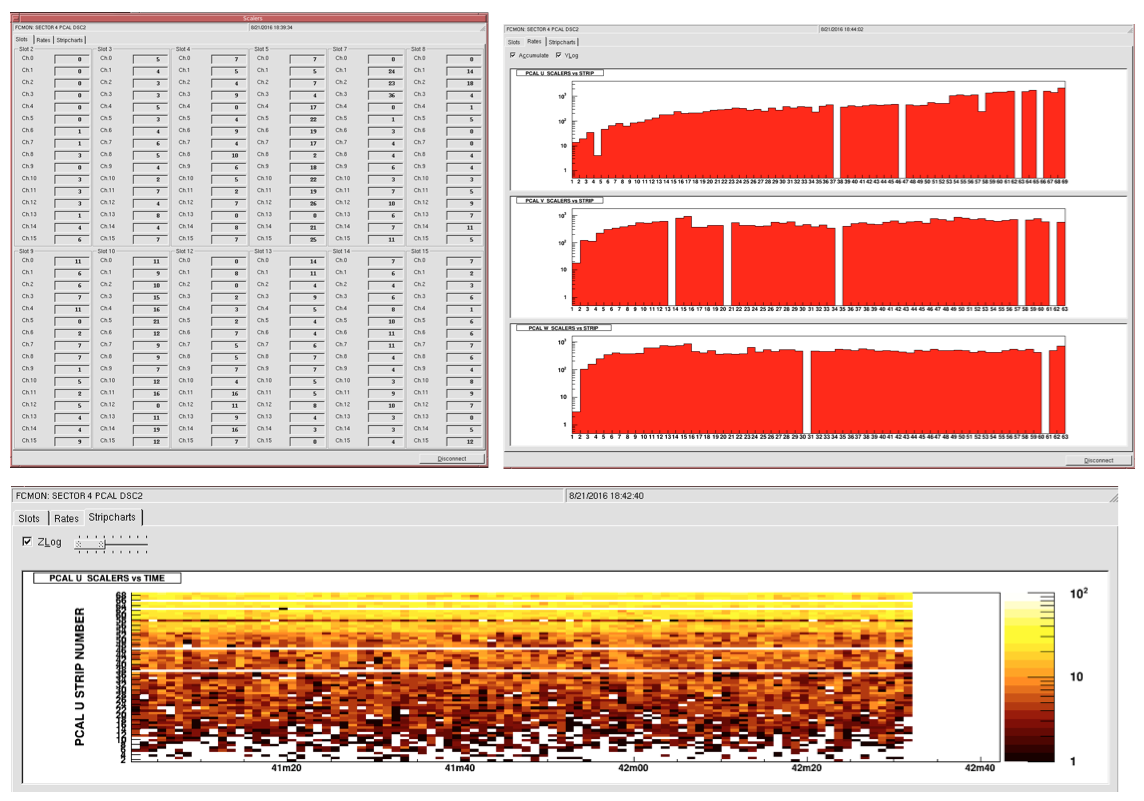
\includegraphics[width= 7in, keepaspectratio = true]{fcmon-screens}
  \vspace{2mm}
  \caption{Display modes of FCMON Scalers GUI. Top Left: Slot,channel readout Top Right: Rates vs. PMT
    number and U,V,W view Bottom: 2D stripchart showing rates vs. time.}
\label{fcmon2}
\end{figure}
%%%%%%%%%%%%%%%%%%%%%%%%%%%%%%%%%%%%%%%%%%%%%%%%%%%%%%%%%%%%%%%%%%%%%%%%%%%%%%%%%%%%%%%%%%%%%%%%%%%%%

As of the time of writing of this document, FCMON is the most direct tool for determining if the front-end
electronics are receiving the intended signals from the PMTs. If holes show up in these plots, the first step is
to determine if the HV for the affected PMT is on and if the HV divider current is non-zero.  For this purpose, the
HV Control GUIs already discussed can provide this information.  Further steps may be taken to determine the cause
of occupancy problems.  A Java based CLAS12 system monitoring suite that is under development will
represent another tool that the shift worker can use to quickly assess the detector status. Both FCMON and 
other monitoring tools will be running on dedicated terminals in the Hall~B Counting House.

\clearpage

\vfil
\eject

\section{Information for Subsystem Experts}

\subsection{Subsystem Expert Responsibilities}

The EC subsystem experts have several key responsibilities:

\begin{enumerate}
\item Complete hot checkout sign-off before the start of each run period (see Section~\ref{checkout}).
\item Respond to calls on the on-call phone to resolve issues with the EC system that are necessary during
data taking (see Section~\ref{oncall}).
\item Take periodic HV gain calibration runs and adjust the system HV settings (see 
Section~\ref{gain-calib}).
\item Make repairs to the hardware during maintenance periods (see Section~\ref{repairs}).
\end{enumerate}

\subsubsection{Hot Checkout}
\label{checkout}

Prior to the start of each physics running period, each subsystem group leader is responsible to
review the components of their systems to be sure that they are fully operational. This review is
referred to as ``hot checkout''. The hot checkout is an online checklist for each system that
includes a sign-off for all hardware elements of the system (e.g. HV, LV, detectors, gas, pulser).
For the EC system, the hot checkout includes verification that all detectors are operational and
that all signals are present as seen through the scaler displays. Fig.~\ref{hot-co} shows screenshots 
of the hot checkout interface from a development version of the system. Under the heading ``Hall~B
CLAS12 Detector'', open the list for the EC system. All entries for EC must be verified as ready.
Note that often as part of the system checkout before the start of a run period, an initial HV gain 
calibration is completed (see Section~\ref{gain-calib}). Reminders to complete the system hot checkout
will be sent out shortly before the start of a given run period with the required deadline for
completing the work.

%%%%%%%%%%%%%%%%%%%%%%%%%%%%%%%%%%%%%%%%%%%%%%%%%%%%%%%%%%%%%%%%%%%%%%%%%%%%%%%%%%%%%%%%%%%%%%%%%%%%%
\begin{figure}[htbp]
  \centering
  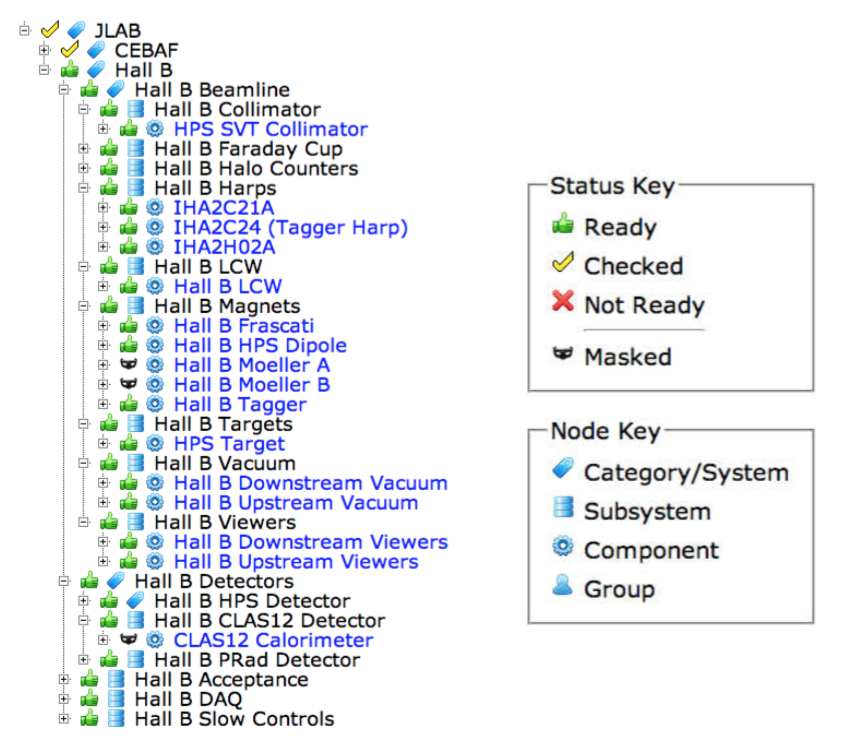
\includegraphics[width= 7in, keepaspectratio = true]{Hot-checkout}
  \vspace{2mm}
\caption{Screenshots of the development version of the Hall~B hot checkout screens. The EC system
will appear under the ``Hall~B CLAS12 Detector'' heading. All entries for EC have been to verified
as functional and all items listed as ``Not Ready'' must be changed over to ``Ready''.}
\label{hot-co}
\end{figure}
%%%%%%%%%%%%%%%%%%%%%%%%%%%%%%%%%%%%%%%%%%%%%%%%%%%%%%%%%%%%%%%%%%%%%%%%%%%%%%%%%%%%%%%%%%%%%%%%%%%%%

\subsubsection{On-call Responsibilities}
\label{oncall}

Each subsystem will organize a list of on-call experts who will take responsibility for carrying
a cell phone to allow 24 hour access to experts who can address any problems that arise during
the physics running period. The phone numbers of all subsystem experts are posted on the run page. 
Any problems that cannot be quickly solved by the shift workers, where quickly amounts to 10 to 15 
minutes, should result in a call to the relevant expert cell phone. 

The on-call experts can often diagnose problems over the telephone, but there are times where they
will have to go to the Counting House to more fully address the issues. One of the important
responsibilities of the on-call experts is to make practical decisions regarding which problems 
require access to Hall~B for immediate attention and when they can be delayed to periods when the 
accelerator is down or other work is scheduled in the hall. For the EC system, usually problems 
with a single channel are not important enough to stop the data acquisition. The normal mode of 
operation after initial investigation of a bad channel, is to turn off the HV for that channel 
until access can be made for a more detailed investigation. This work should be coordinated with
the Run Coordinator.

Note: It is the responsibility of the EC on-call expert to review all issues that they cannot
resolve with the EC subsystem Group Leader as soon as is reasonable.

\subsubsection{HV Gain Calibrations}
\label{gain-calib}

The HV gain calibrations for the EC system are typically completed before the start of each run
period, as well as several times during the run period when there is opportunity. The HV gain 
calibration procedure employs a cosmic ray trigger defined either ECAL or PCAL. 
The ADC spectra for each counter are fit to ensure that the minimum ionizing particle peak appears 
at a specific location in the ADC range corresponding to a specific gain. The end result of the 
gain calibration amounts to adjusting the system HV settings to position the ADC peaks at their 
assigned locations.

The calibration suite for the EC system includes both an online and an offline component. The
online component is used to calibrate the PMT gains and the output is a table of PMT HV settings
that are downloaded into the HV power supplies. The offline component is used to determine the
parameters to optimize the absolute energy calibration and resolution of the system. Full documentation
on using EC calibration, including tutorials for using the code, are included on the EC web page.
\cite{ecal-web}.


\subsection{HV System Operations}

\subsubsection{Setting HV Channel Parameters}
\label{hv-parms}

The CS-Studio program is used to monitor the HV settings of the EC system and to toggle the HV off
and on for individual or multiple channels in the system.  As discussed in Section~\ref{hv-control}, there is also
the option to adjust settings channel-by-channel using the HV ``expert'' screen shown in
Fig.~\ref{ecal-screen3}. Here the parameters, $V_{set}$, $I_{set}$, $V_{max}$, and the HV ramp up and
ramp down rates, can be entered directly into the parameter fields.  This ``expert'' screen
should most properly be used only for viewing the channel parameter set values. Finally there are control scripts
available in the event nominal settings need to be restored. From the computers in the Hall~B Counting House,
the scripts are located in the sector subdirectories located in the path: {\it /home/clasrun/ecal/hv/sn}, and
{\it /home/clasrun/pcal/hv/sn} where {\it sn} corresponds to {\it s1} to {\it s6} for S1 $\to$ S6.
There are five scripts available for setting these HV channel parameters:

\begin{itemize}
\item {\it loadhvmax-sn}: Maximum HV limits for each supply channel (units = V)
\item {\it loadi0-sn}:    Maximum current limits for each supply channel (units = $\mu$A)
\item {\it loadrup-sn}:   Voltage ramp up rates for each supply channel (units = V/s)
\item {\it loadrdn-sn}:   Voltage ramp down rates for each supply channel (units = V/s)
\item {\it loadtrip-sn}:  Maximum time duration for an overcurrent condition before the 
channel trips (units = s)
\end{itemize}

The nominal settings for the HV channel parameters are as follows:

\begin{itemize}
\item HV values (PCAL): Typically in the range from -800~V to -950~V
\item HV values (ECAL): Typically in the range from -1500~V to -2000~V
\item HV values (PCAL): Typically in the range from -800~V to -950~V
\item HV$_{max}$ values: PCAL: -1100~V, ECAL: -2500~V
\item i$_{max}$ values: 500~$\mu$A
\item HV ramp up rate: 50~V/s
\item HV ramp down rate: 100~V/s
\item Overcurrent duration before trip: 1~s
\end{itemize}

Individual HV values and the enable/disable status of each PMT are created by the monitoring and
calibration programs and these values are stored in a separate database.  There are no backup scripts for
setting these values since they are time-dependent and have to be carefully managed.  Nevertheless
save and restore values can be archived from the EC HV control screen (see Section~\ref{save-restore}.


\subsubsection{HV Save and Restore}
\label{save-restore}

The EC HV interface allows all system channel settings to be saved into a file or loaded from an
archived file by clicking on the ``ECAL'' or ``PCAL'' button in the upper right corner of the main HV
screen (see Fig.~\ref{ecal-screen}). The files created are referred to as ``BURT'' backup files,
where BURT is an acronym for ``Backup and Restore Tool''. BURT is a utility for saving the HV system
settings into an ascii file readable by the EPICS Slow Control system.

After clicking on the detector button, a sub-menu appears as shown in Fig.~\ref{backup-restore1}
to select ``Save Settings'' or ``Restore Settings''. Clicking on ``Save Settings'' brings up a window
``CREATE HV BACKUP'' as shown at bottom,  displaying the save file path and the selected
file name that contains the system name along with the date and time. If the ``Restore Settings'' option
is chosen, the window shown in Fig.~\ref{backup-restore2} comes up showing the saved ECAL or PCAL  HV restore
files available to select from. Selecting a file and clicking on ``OK'' at the bottom of the window
loads all channel parameters for the full HV system. Note that a new backup file should be created 
whenever any HV settings have changed, including HV values, channel parameter settings, and channel 
on/off settings.

%%%%%%%%%%%%%%%%%%%%%%%%%%%%%%%%%%%%%%%%%%%%%%%%%%%%%%%%%%%%%%%%%%%%%%%%%%%%%%%%%%%%%%%%%%%%%%%%%%%%%
\begin{figure}[htbp]
  \centering
  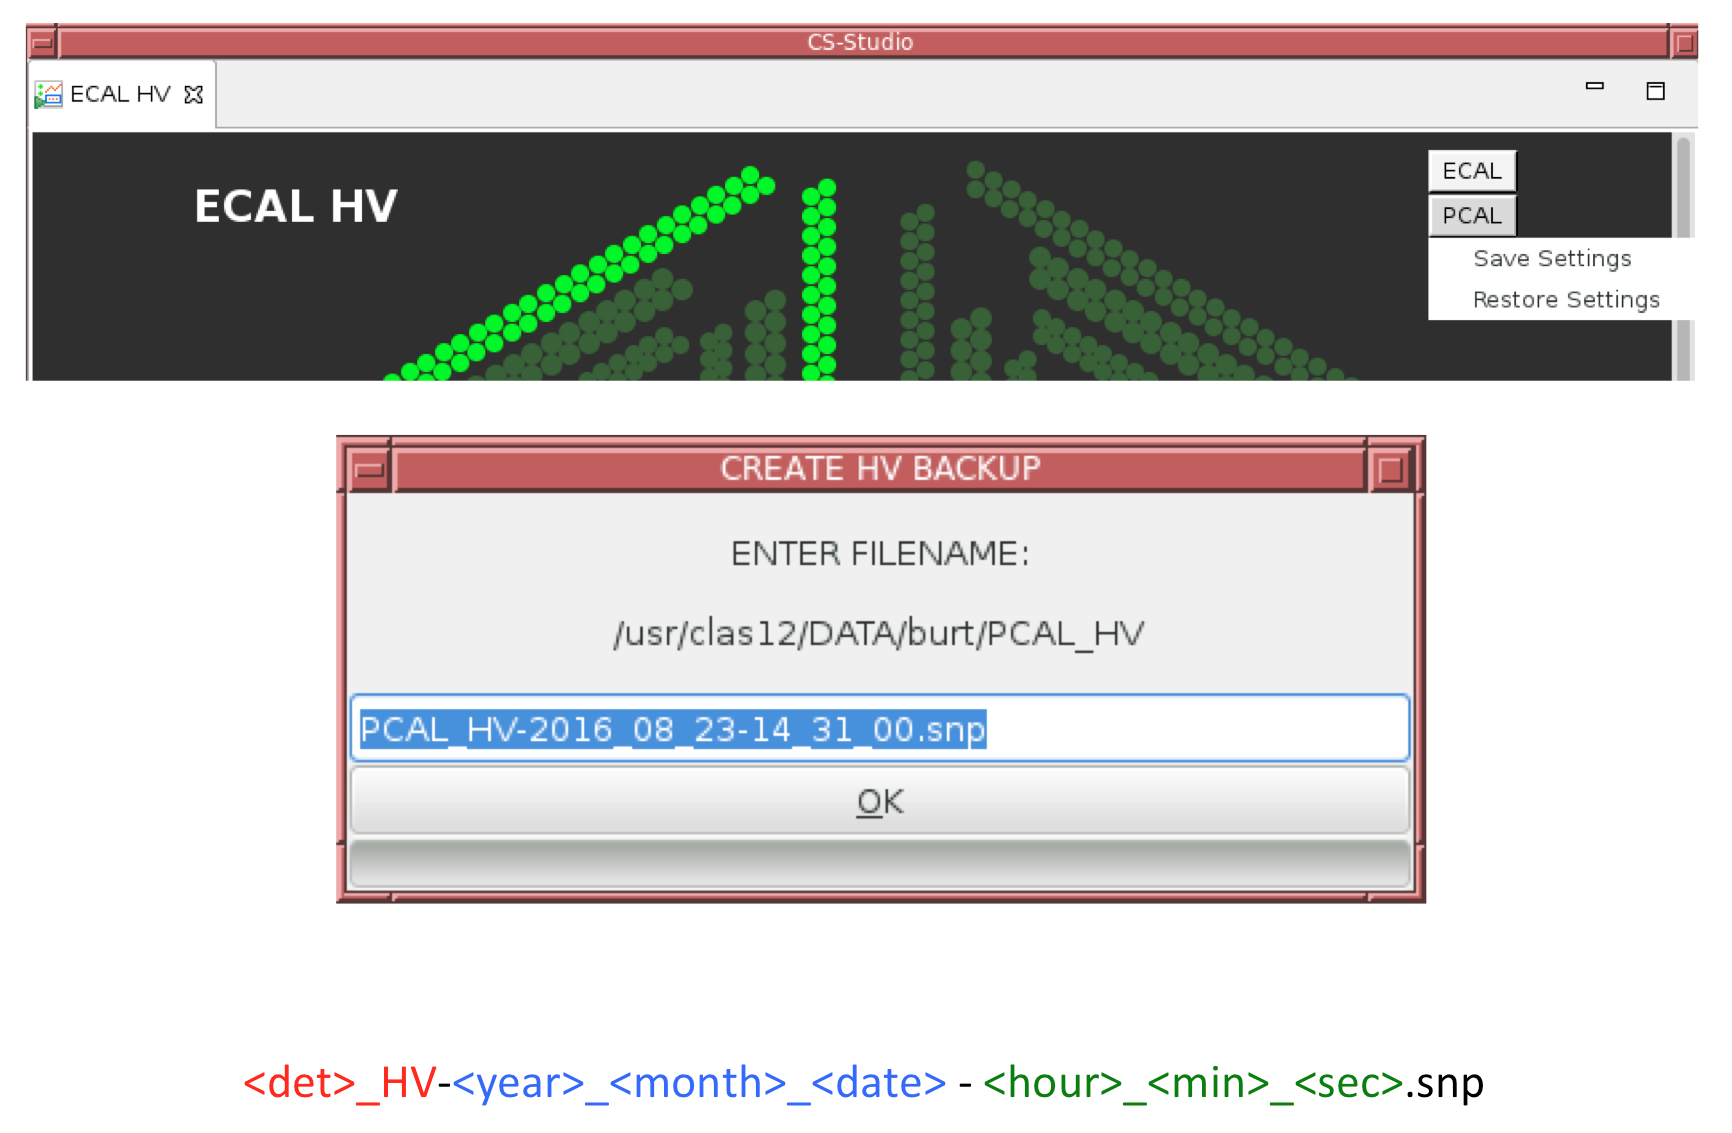
\includegraphics[width= 5in, keepaspectratio = true]{burt-save.png}
  \vspace{2mm}
  \caption{Top: Choose the appropriate detector (ECAL or PCAL) for saving HV settings.  The pop-up menu will
    allow you to select ``Save Settings'' or ``Restore Settings''.  Bottom: If ``Save Settings'' is chosen,
    a pop-up confirmation dialog will display the path and name of the BURT snapshot file, using the timestamp format shown at bottom.
    This name can be edited if desired.}
\label{backup-restore1}
\end{figure}
%%%%%%%%%%%%%%%%%%%%%%%%%%%%%%%%%%%%%%%%%%%%%%%%%%%%%%%%%%%%%%%%%%%%%%%%%%%%%%%%%%%%%%%%%%%%%%%%%%%%%
%%%%%%%%%%%%%%%%%%%%%%%%%%%%%%%%%%%%%%%%%%%%%%%%%%%%%%%%%%%%%%%%%%%%%%%%%%%%%%%%%%%%%%%%%%%%%%%%%%%%%
\begin{figure}[htbp]
  \centering
  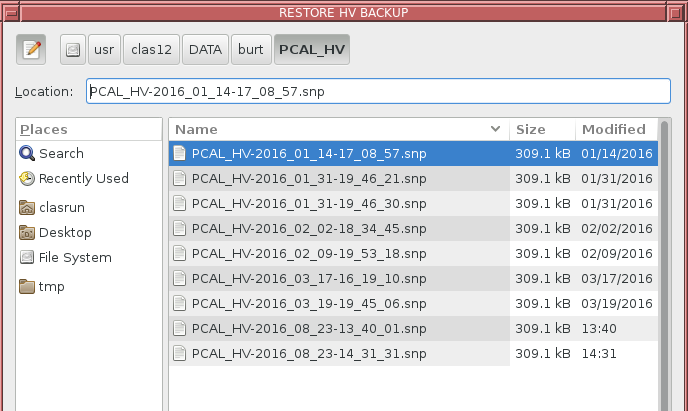
\includegraphics[width= 5in, keepaspectratio = true]{burt-restore.png}
  \vspace{2mm}
  \caption{If ``Restore Settings'' is chosen, use the pop-up file chooser to select the snapshot
    file for restoring HV settings.}
\label{backup-restore2}
\end{figure}
%%%%%%%%%%%%%%%%%%%%%%%%%%%%%%%%%%%%%%%%%%%%%%%%%%%%%%%%%%%%%%%%%%%%%%%%%%%%%%%%%%%%%%%%%%%%%%%%%%%%%
\subsection{Cabling Details}

\subsubsection{Signal Cable Layout}
\label{signal-conn}

The U,V,W PMTs for the ECAL modules are located at the rear (downstream) face of each triangle-shaped module
(see Figure~\ref{ecal-pmts}) and are distributed uniformly along its perimeter.  There are two layers of
PMTs: the top layer reads out the inner calorimeter (closest to the target) and the bottom layer reads out
the outer calorimeter. The PMTs are also oriented
parallel to the U,V,W strips within each module.  HV and RG-8 signal cables are fastened to and routed along steel gratings
running parallel to the calorimeter sides.  RG-58 patch cables (16 ns delay) run from the PMT anode connector
to the thicker and less flexible RG-8 cable.  At the other end of the RG-8, a second connection is made to
RG-58 patch cables (16 ns delay) connected to LEMO inputs at the rear of the UVA 122B splitter panels.  These
patch connections are illustrated by the photos in Figures~\ref{ecal-patch-cables} and \ref{fc-layout-3}.

%%%%%%%%%%%%%%%%%%%%%%%%%%%%%%%%%%%%%%%%%%%%%%%%%%%%%%%%%%%%%%%%%%%%%%%%%%%%%%%%%%%%%%%%%%%%%%%%%%%%
\begin{figure}[htbp]
  \centering
  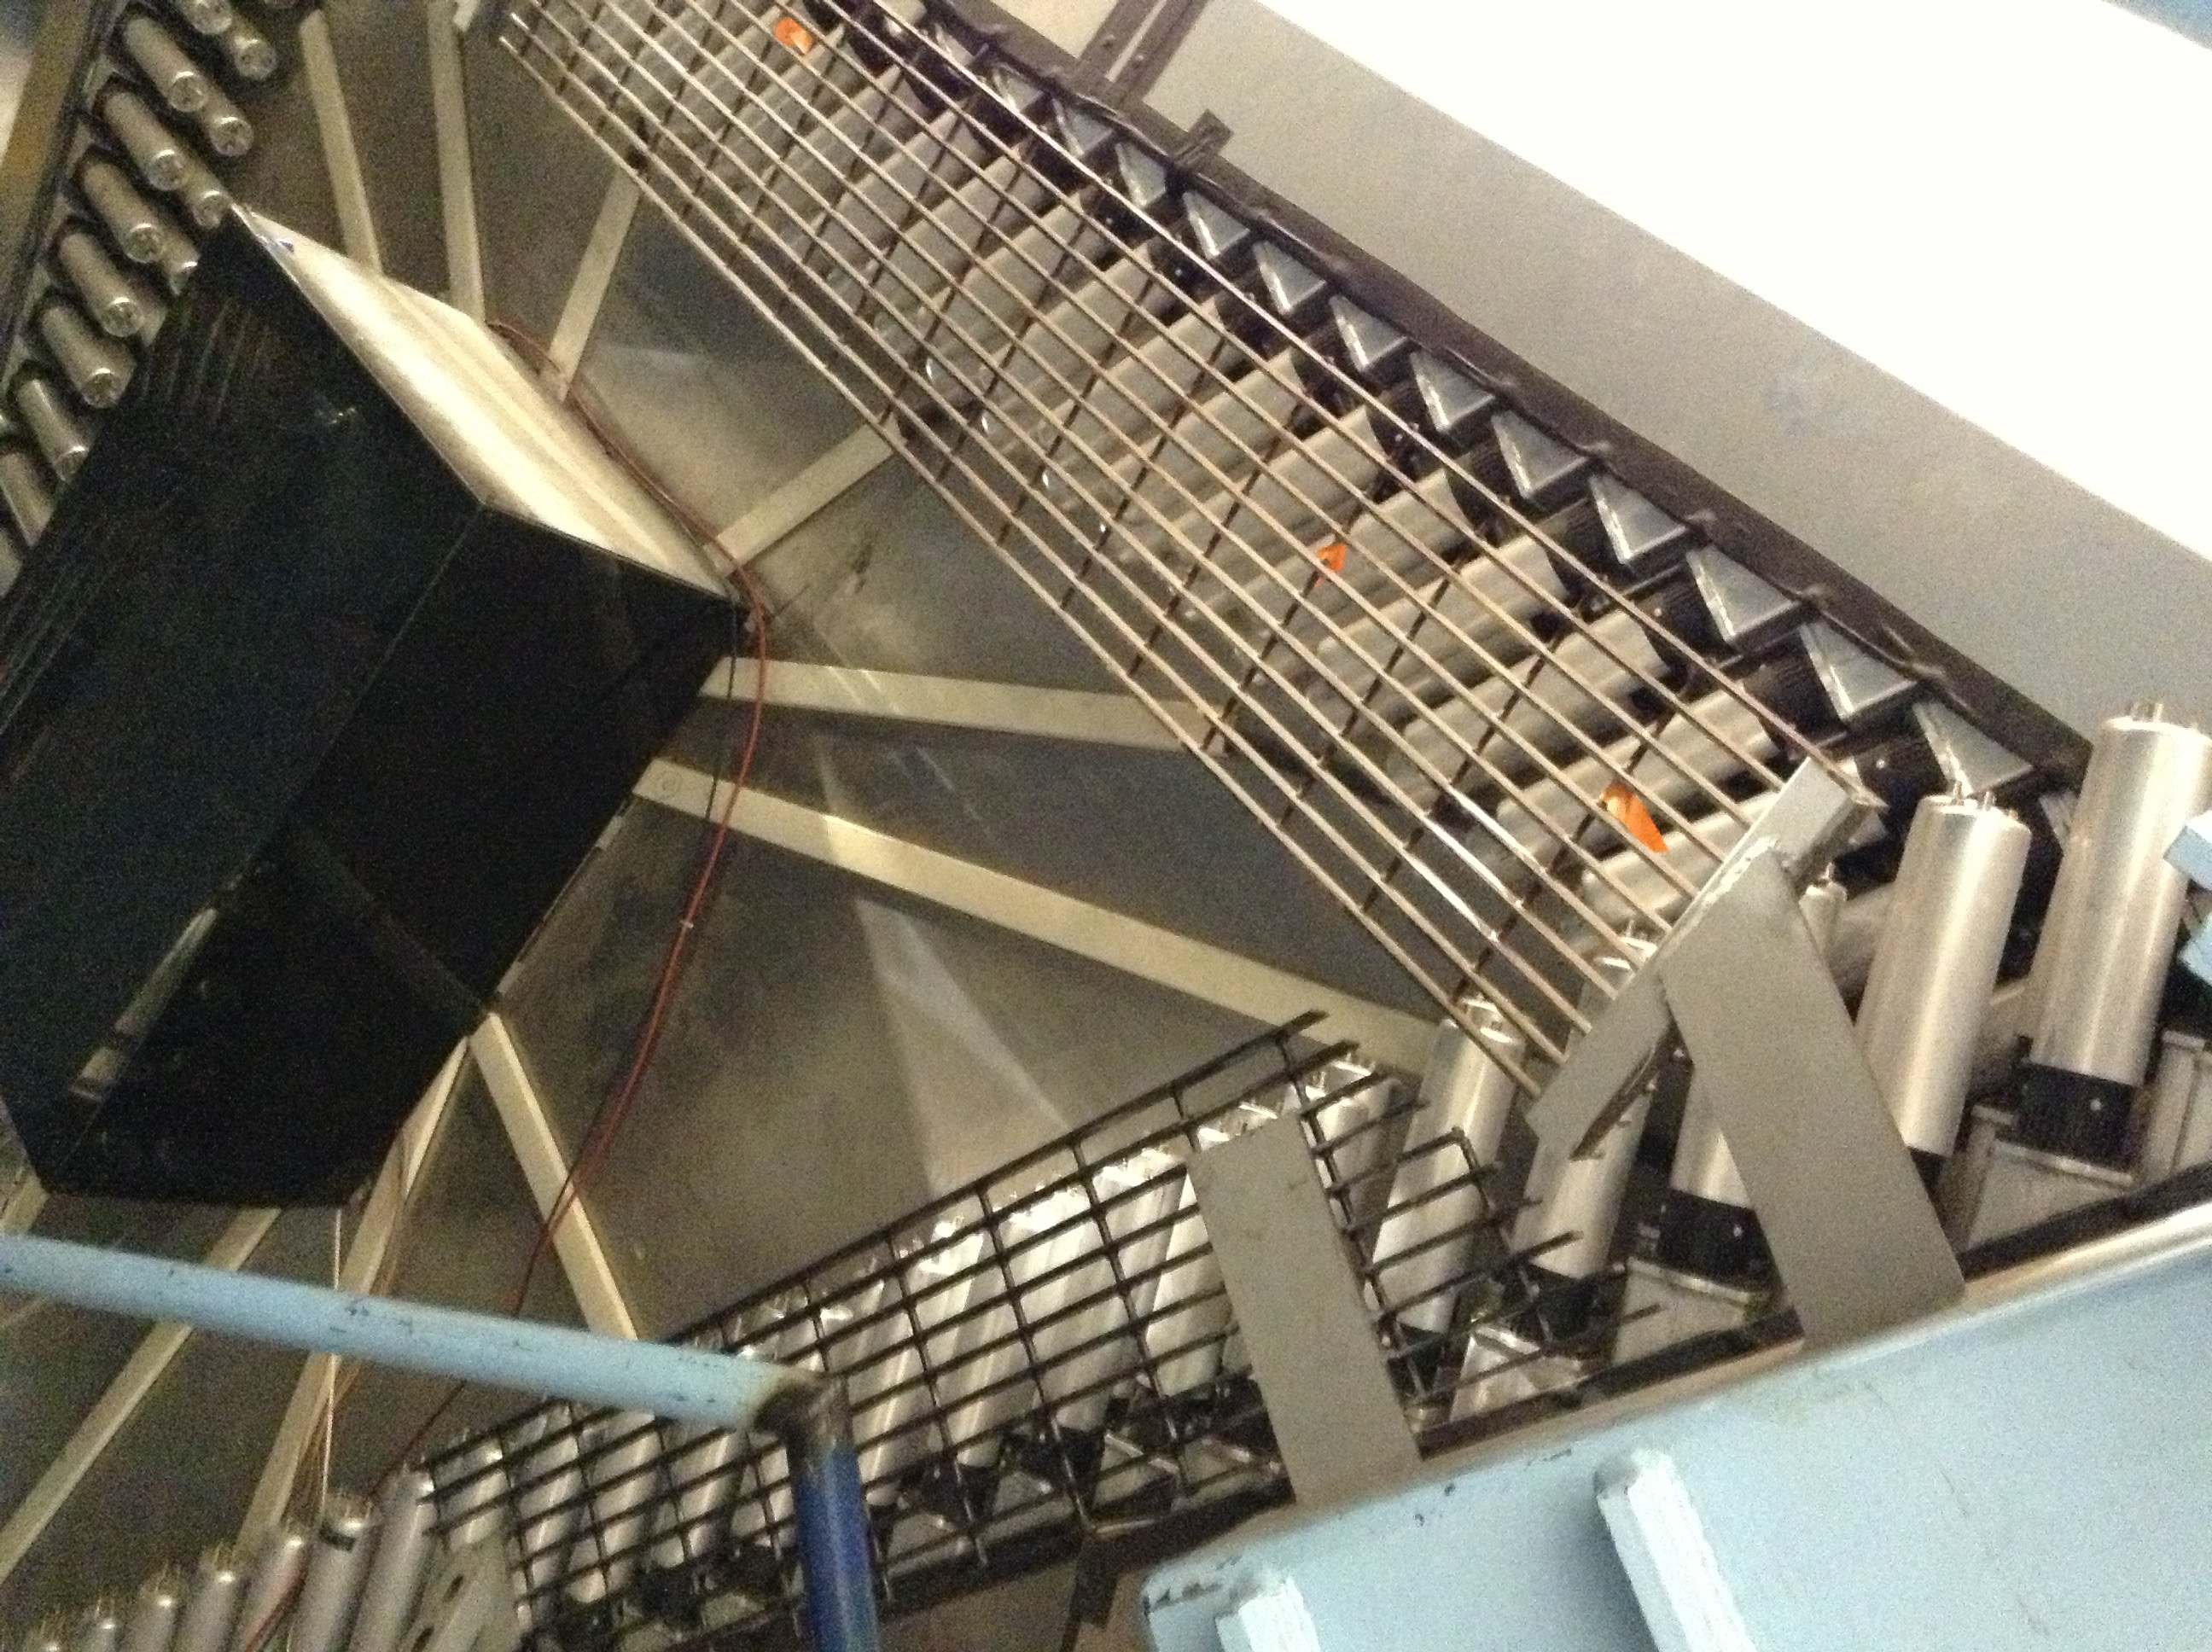
\includegraphics[width= 5in, keepaspectratio = true]{ecal-pmts.jpg}
  \vspace{2mm}
  \caption{Placement of ECAL U,V,W PMTs at rear (downstream) side of Sector 2 module.  Gratings are
  used to route HV and RG-8 signal cables.}
\label{ecal-pmts}
\end{figure}
%%%%%%%%%%%%%%%%%%%%%%%%%%%%%%%%%%%%%%%%%%%%%%%%%%%%%%%%%%%%%%%%%%%%%%%%%%%%%%%%%%%%%%%%%%%%%%%%%%%%%


%%%%%%%%%%%%%%%%%%%%%%%%%%%%%%%%%%%%%%%%%%%%%%%%%%%%%%%%%%%%%%%%%%%%%%%%%%%%%%%%%%%%%%%%%%%%%%%%%%%%
\begin{figure}[htbp]
  \centering
  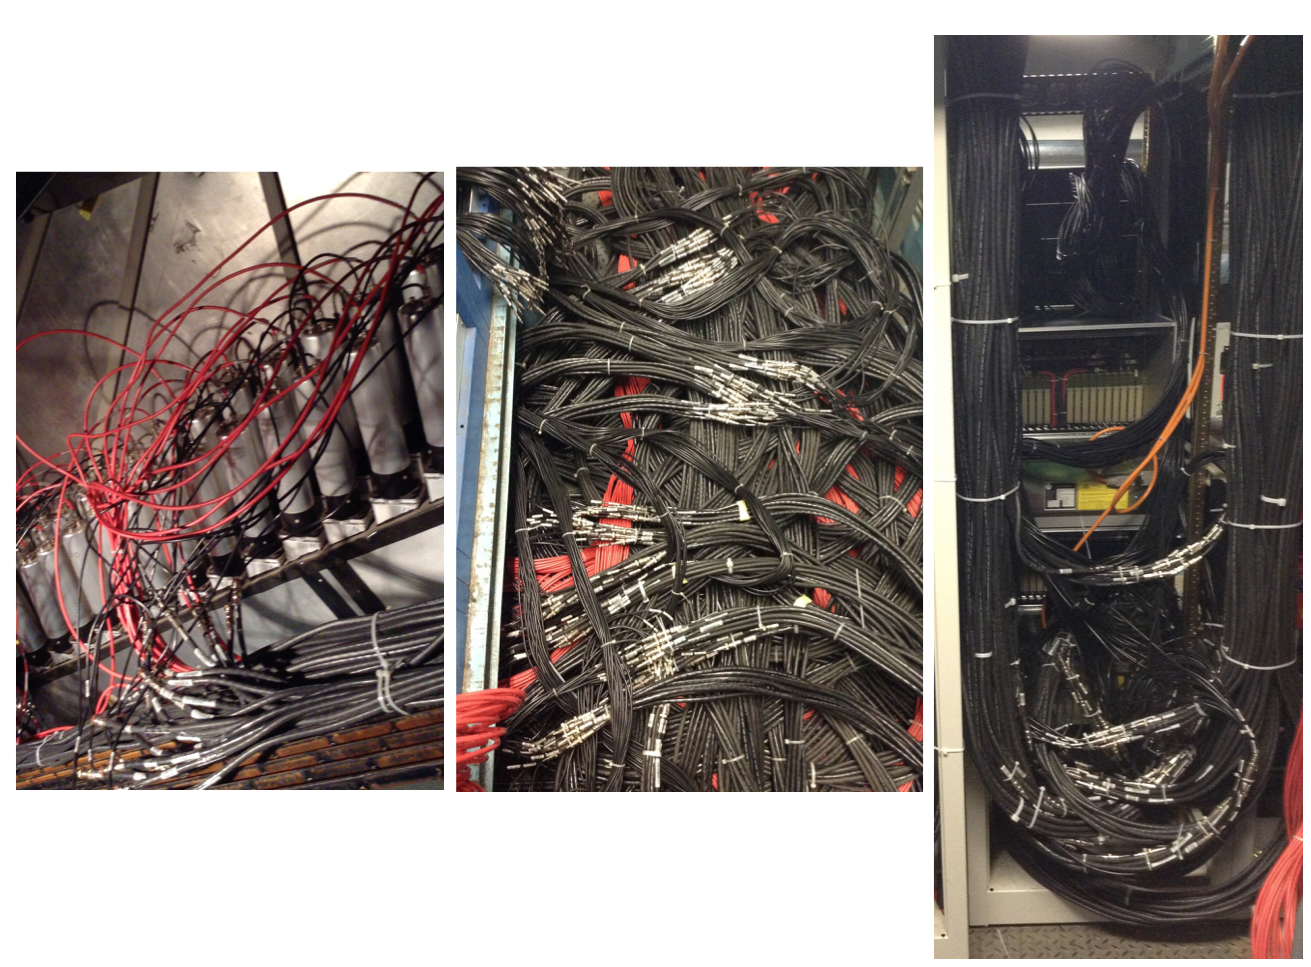
\includegraphics[width= 7in, keepaspectratio = true]{ecal-patch-cables.png}
  \vspace{2mm}
  \caption{For ECAL two RG-58 16 ns patch cable connections are made to the RG-8 signal cable: at the PMT
    end and near the UVA 122B splitter panels at the electronic racks.  Left: Connections
    made along the rail grating next to the PMTs.  Middle: Connection made beneath the floor gratings on
    Levels 2 and 3 of the Forward Carriage.  Right: Connections made within the electronics racks on Level 1.}
\label{ecal-patch-cables}
\end{figure}
%%%%%%%%%%%%%%%%%%%%%%%%%%%%%%%%%%%%%%%%%%%%%%%%%%%%%%%%%%%%%%%%%%%%%%%%%%%%%%%%%%%%%%%%%%%%%%%%%%%%%

The U,V,W PMTs for the PCAL modules are mounted along the sides of each module
(see Figures~\ref{pcal-pmts} and \ref{pcal-pmts-2}).  Due to geometry constraints the V,W PMTs for PCAL are located
together on the same side (corresponding to V PMT side of the ECAL.)  For PCAL only the U PMTs and cable connections
are accessible from the Forward Carriage decks.  Figure~\ref{pcal-pmts-3} shows a view of the PCAL U cable routing
within the gap between adjacent ECAL modules, and Figure~\ref{pcal-pmts-4} shows the V,W cable routing for Sector 6.
No patch cables are used for PCAL.  The RG-58 signal cables have a BNC connector on the PMT end and a
LEMO connector on the splitter panel end.


%%%%%%%%%%%%%%%%%%%%%%%%%%%%%%%%%%%%%%%%%%%%%%%%%%%%%%%%%%%%%%%%%%%%%%%%%%%%%%%%%%%%%%%%%%%%%%%%%%%%
\begin{figure}[htbp]
  \centering
  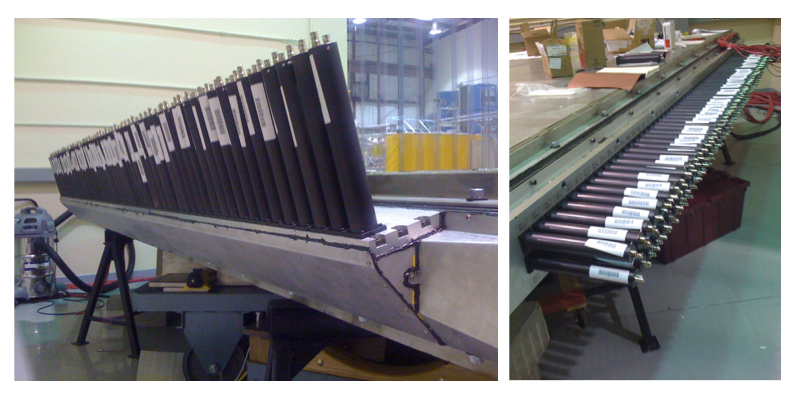
\includegraphics[width= 5in, keepaspectratio = true]{pcal-pmts}
  \vspace{2mm}
  \caption{Placement of PCAL U PMTs (left) and V,W PMTs (right).  Photo taken in EEL Building. }
\label{pcal-pmts}
\end{figure}
%%%%%%%%%%%%%%%%%%%%%%%%%%%%%%%%%%%%%%%%%%%%%%%%%%%%%%%%%%%%%%%%%%%%%%%%%%%%%%%%%%%%%%%%%%%%%%%%%%%%%

%%%%%%%%%%%%%%%%%%%%%%%%%%%%%%%%%%%%%%%%%%%%%%%%%%%%%%%%%%%%%%%%%%%%%%%%%%%%%%%%%%%%%%%%%%%%%%%%%%%%
\begin{figure}[htbp]
  \centering
  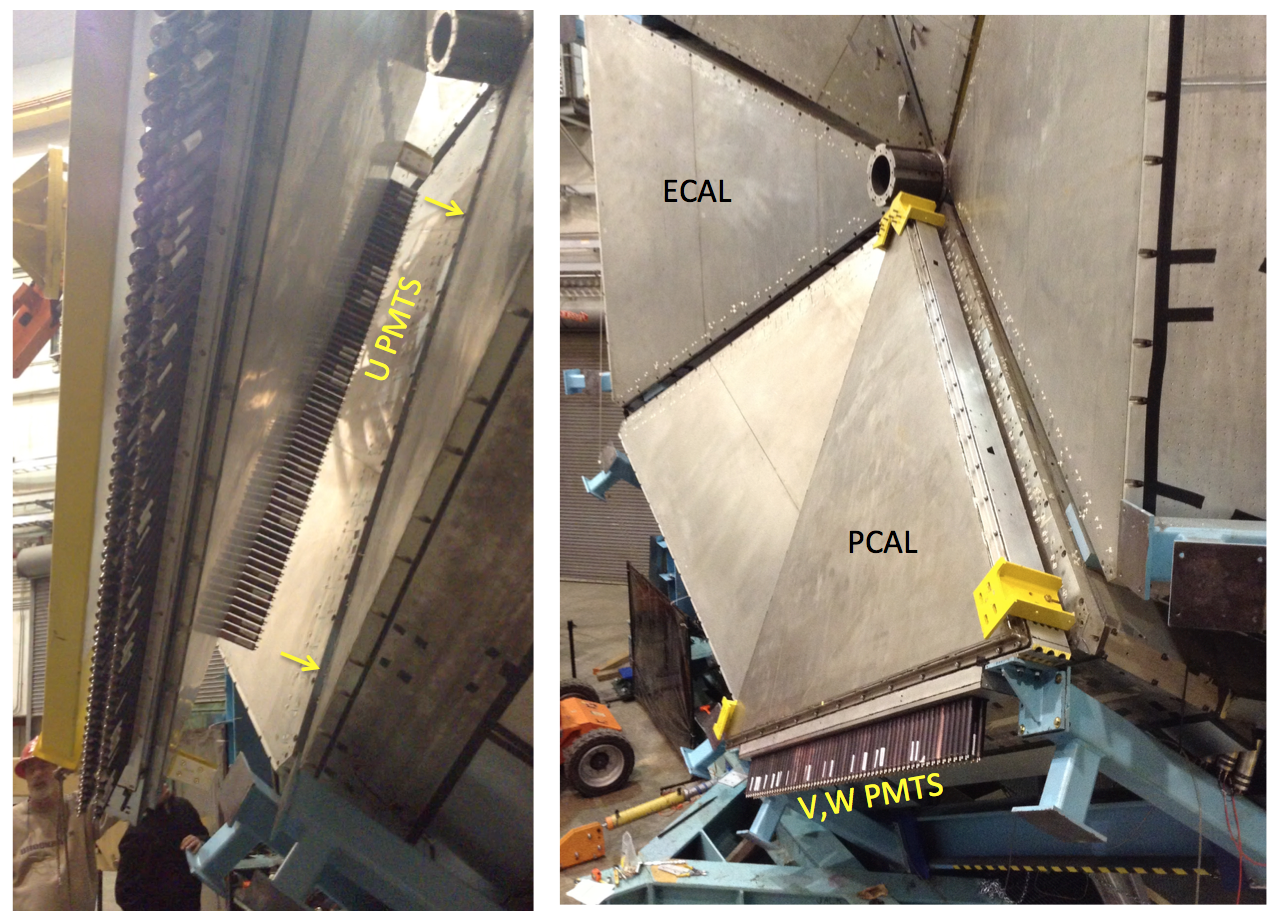
\includegraphics[width= 5in, keepaspectratio = true]{pcal-installation}
  \vspace{2mm}
  \caption{Orientation of PCAL U and V,W PMTs relative to ECAL.  Photo taken in Hall B during installation
  of PCAL in Sector 5 of the Forward Carriage.}
\label{pcal-pmts-2}
\end{figure}
%%%%%%%%%%%%%%%%%%%%%%%%%%%%%%%%%%%%%%%%%%%%%%%%%%%%%%%%%%%%%%%%%%%%%%%%%%%%%%%%%%%%%%%%%%%%%%%%%%%%%

%%%%%%%%%%%%%%%%%%%%%%%%%%%%%%%%%%%%%%%%%%%%%%%%%%%%%%%%%%%%%%%%%%%%%%%%%%%%%%%%%%%%%%%%%%%%%%%%%%%%
\begin{figure}[htbp]
  \centering
  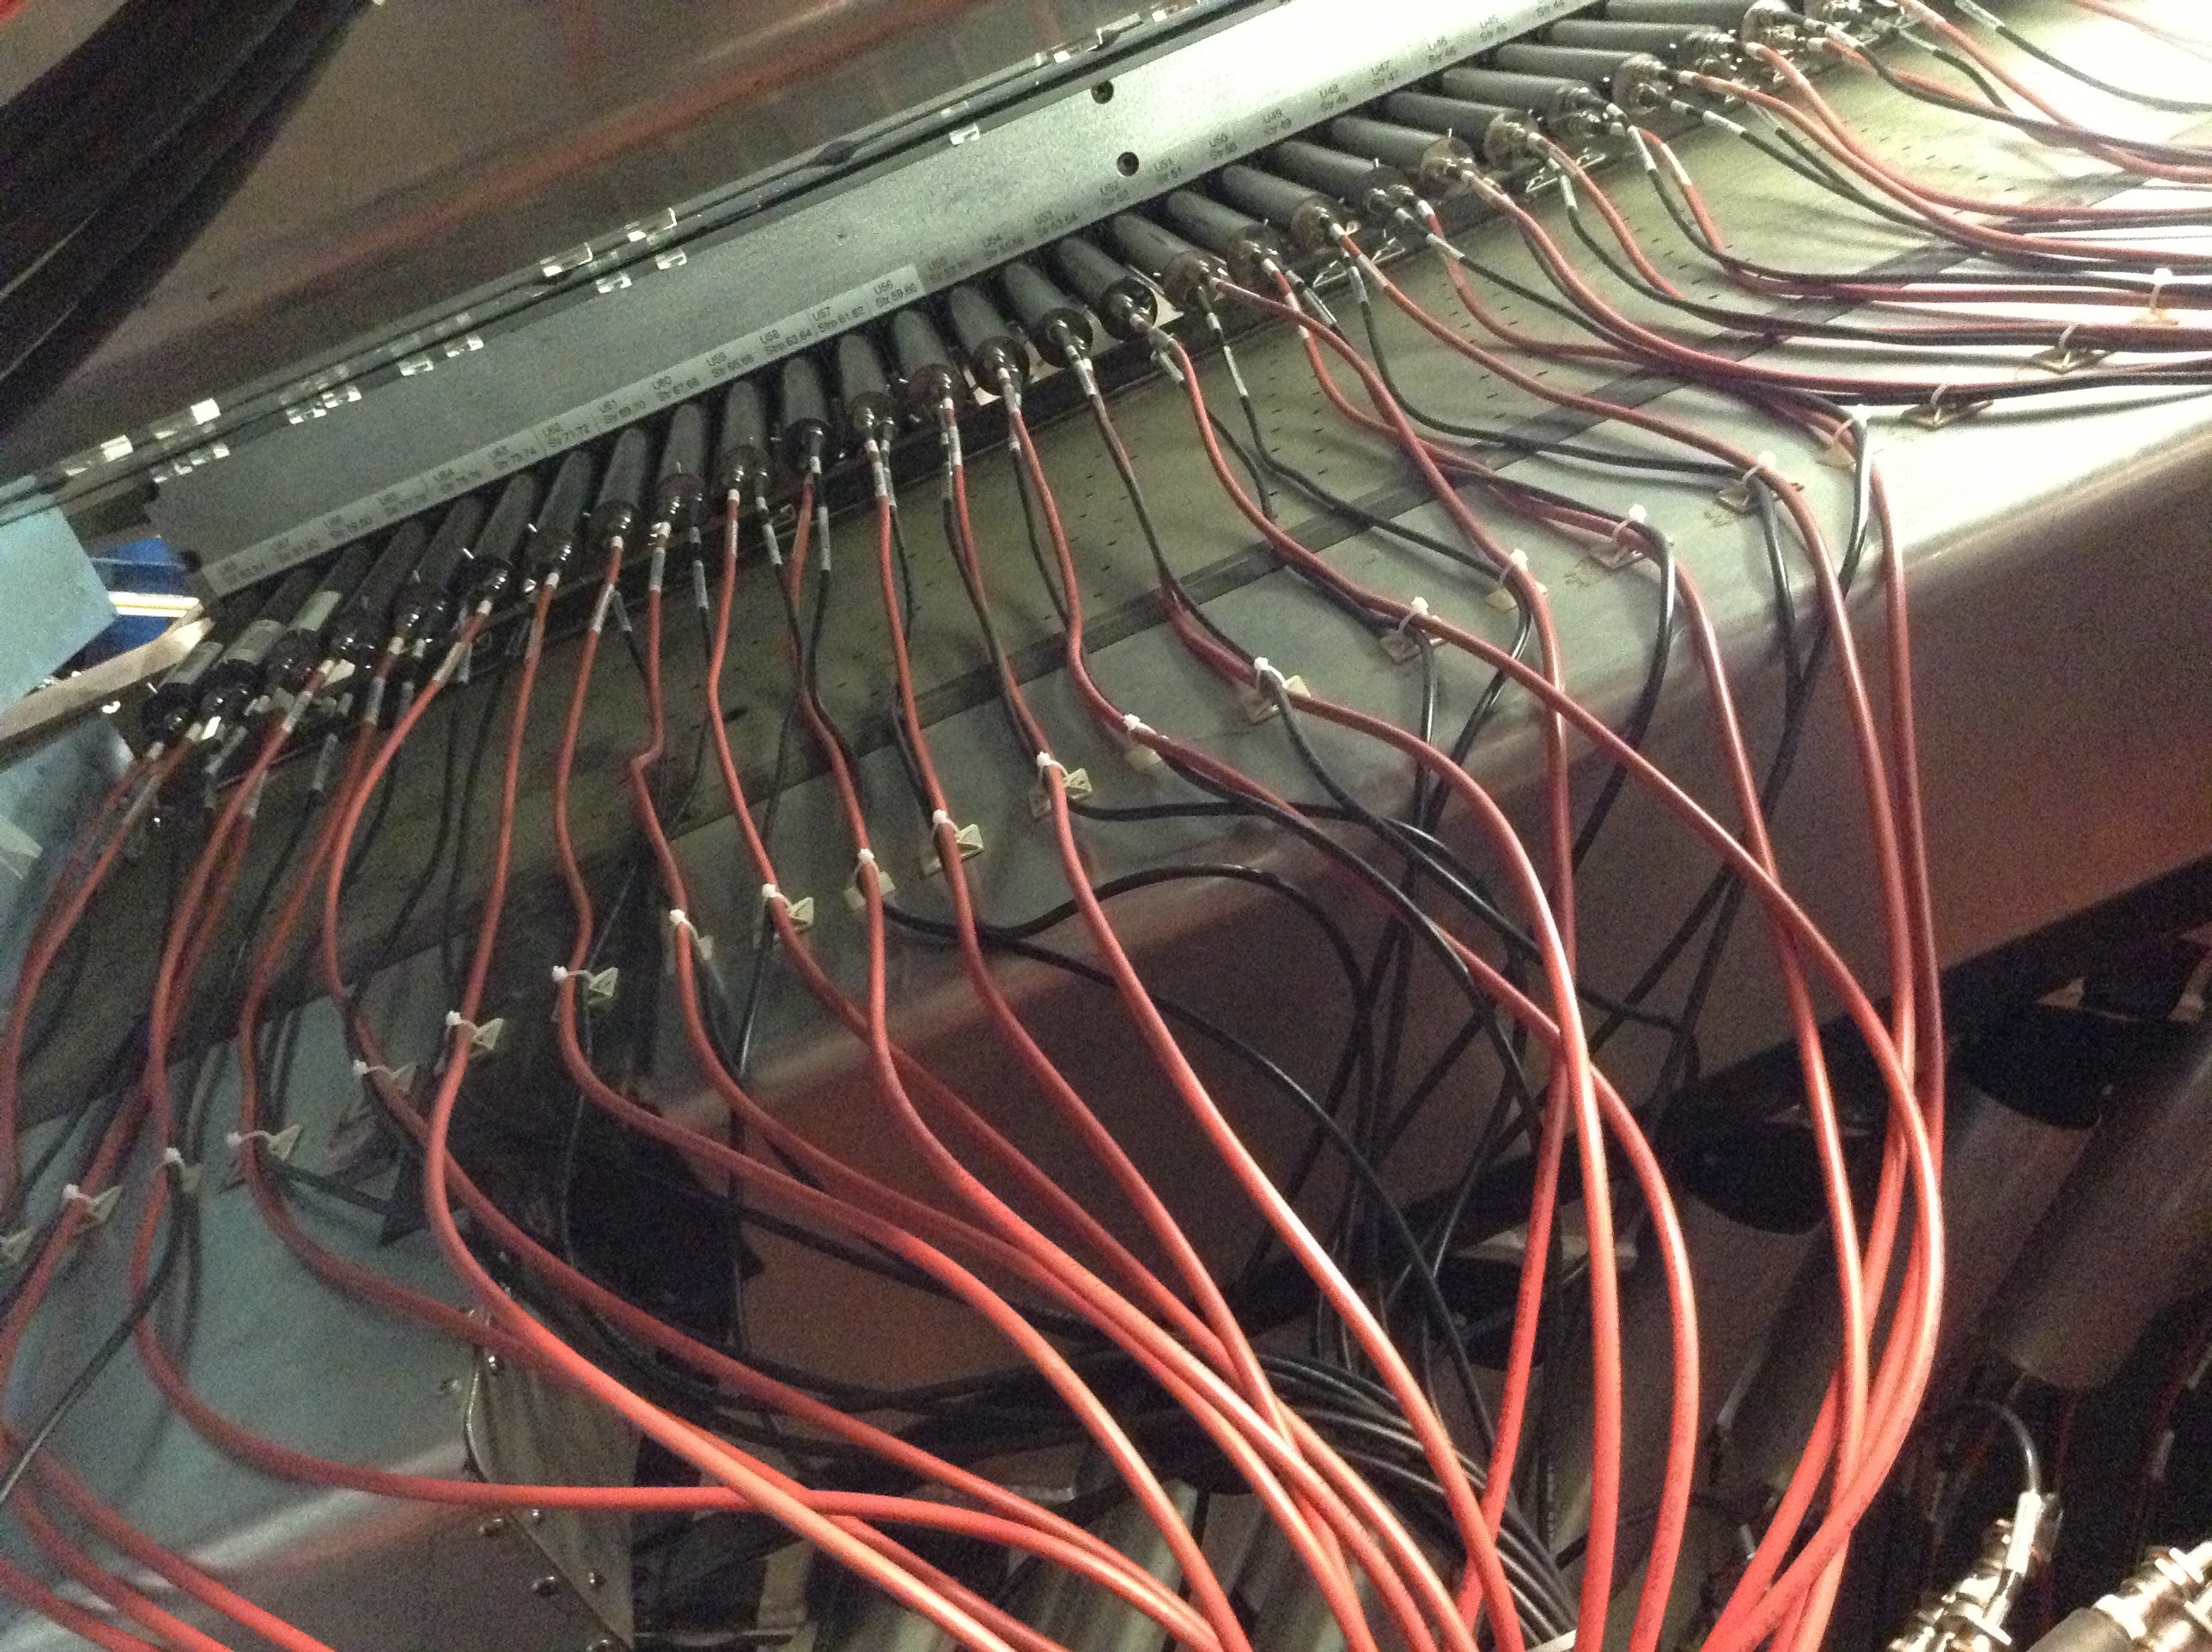
\includegraphics[width= 5in, keepaspectratio = true]{pcal-installation-3.jpg}
  \vspace{2mm}
  \caption{Routing of HV and RG-58 signal cables from U PMTs of PCAL.  Cables pass through the
  gap in between adjacent ECAL modules (seen above and below in the photo.)}
\label{pcal-pmts-3}
\end{figure}
%%%%%%%%%%%%%%%%%%%%%%%%%%%%%%%%%%%%%%%%%%%%%%%%%%%%%%%%%%%%%%%%%%%%%%%%%%%%%%%%%%%%%%%%%%%%%%%%%%%%%

%%%%%%%%%%%%%%%%%%%%%%%%%%%%%%%%%%%%%%%%%%%%%%%%%%%%%%%%%%%%%%%%%%%%%%%%%%%%%%%%%%%%%%%%%%%%%%%%%%%%
\begin{figure}[htbp]
  \centering
  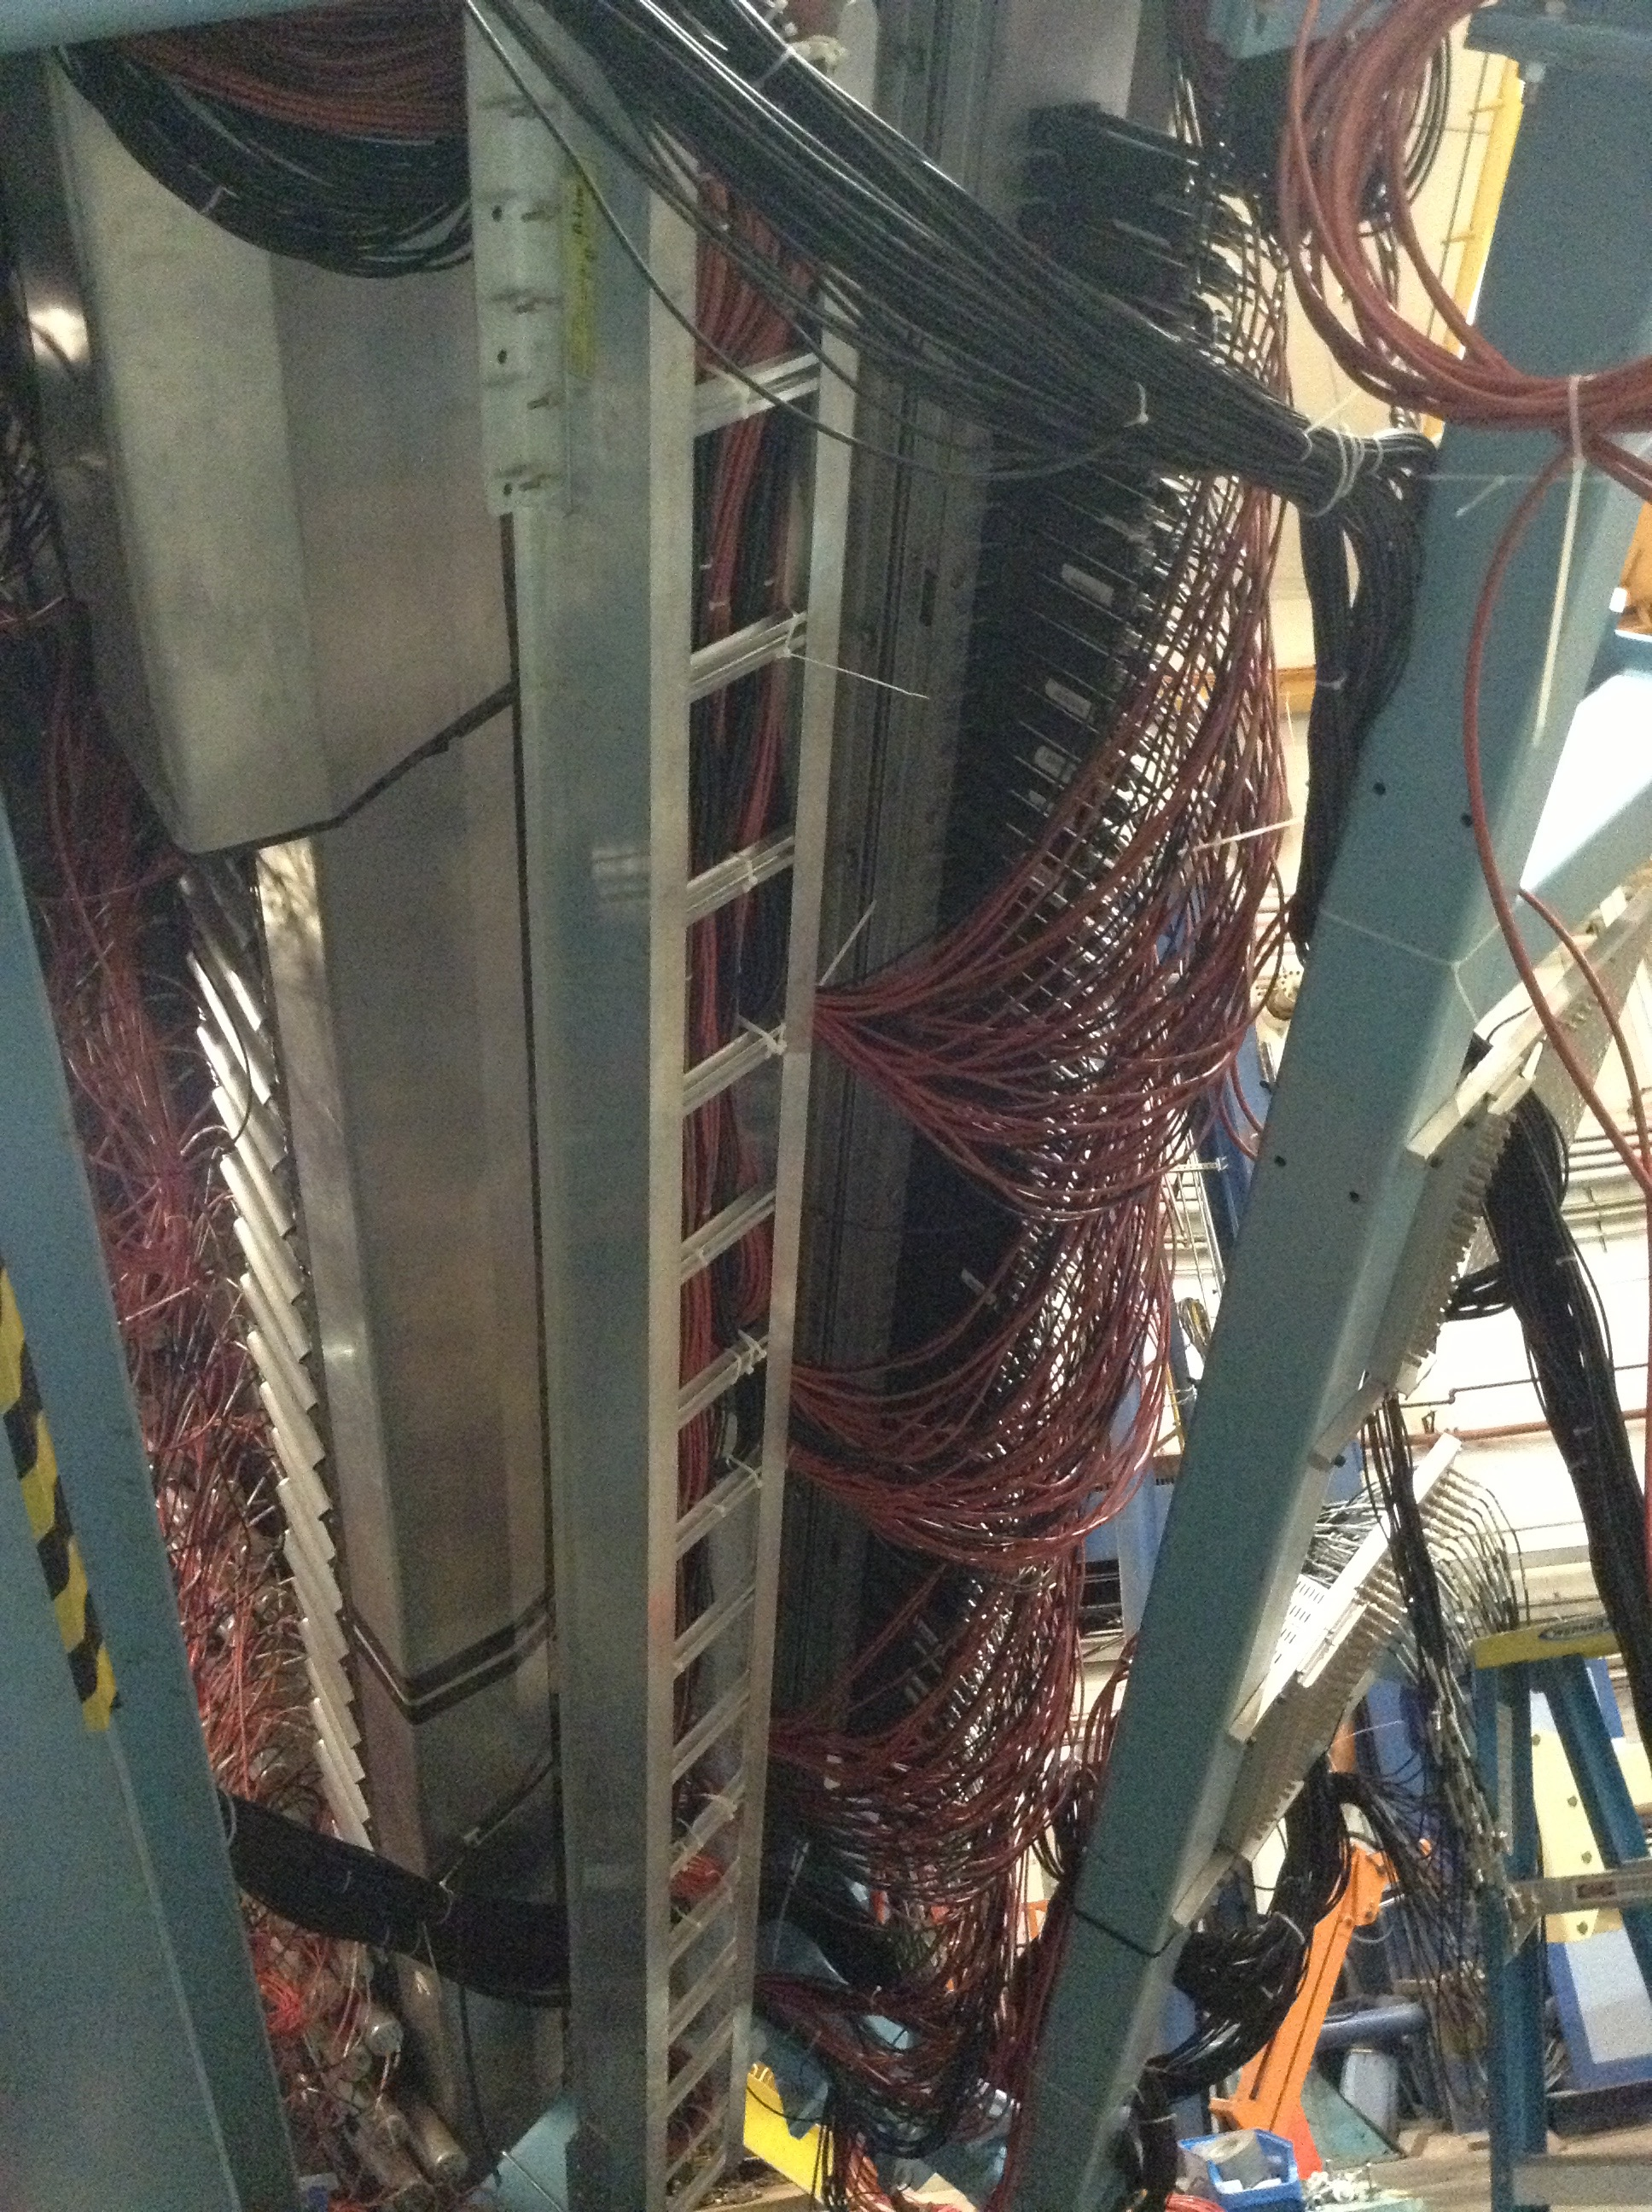
\includegraphics[width= 5in, keepaspectratio = true]{pcal-installation-4.jpg}
  \vspace{2mm}
  \caption{Routing of HV and RG-58 signal cables from V,W PMTs of PCAL.  Cables are routed directly to
    cable trays mounted parallel to the V,W readout side for all modules. Only Sector 5 and Sector 6
    (seen here) V,W PMTs are accessible from floor level with ladders.  Other sectors require a man-lift for access.
     Also visible at left are the V PMTs for ECAL.}
\label{pcal-pmts-4}
\end{figure}
%%%%%%%%%%%%%%%%%%%%%%%%%%%%%%%%%%%%%%%%%%%%%%%%%%%%%%%%%%%%%%%%%%%%%%%%%%%%%%%%%%%%%%%%%%%%%%%%%%%%%


\subsubsection{HV Cable Layout}
\label{hv-layout}

HV cables generally run parallel or along the same general path as the signal cables for both PCAL and ECAL.
HV cable connections to the rear of the CAEN mainframes are made using a JLAB built transition/distribution
box which has 48 SHV input connectors and two output cables each terminated with a 24-pin Radiall connector
designed to mate with the input connector on the A1535N cards (see Figure~\ref{fc-layout-3}).

Both HV and signal cables from the EC system pass under the floor gratings on Levels 2 and 3.  For Level 1
cables are routed through openings in the ceiling.  Connections to the BNC-Lemo transition cables used for the ECAL
RG-8 cables are made under the grating near the racks containing the ECAL splitter panels.  A photo showing
the floor grating removed is in Figure~\ref{fc-layout-3} (right).

%%%%%%%%%%%%%%%%%%%%%%%%%%%%%%%%%%%%%%%%%%%%%%%%%%%%%%%%%%%%%%%%%%%%%%%%%%%%%%%%%%%%%%%%%%%%%%%%%%%%%
\begin{figure}[htbp]
  \centering
  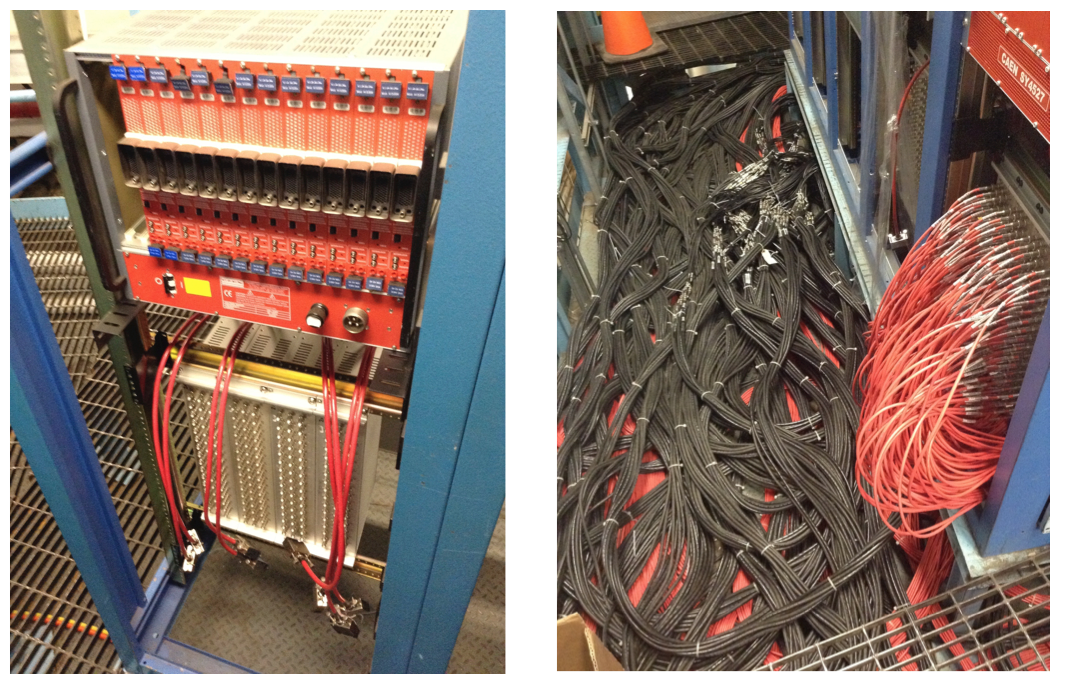
\includegraphics[width= 6in, keepaspectratio = true]{Cable-routing}
  \vspace{2mm}
  \caption{Left: Rear of CAEN HV mainframe (top) showing installed HV cards.  At bottom are transition
    boxes with SHV input connectors and red output cables which mate with the HV cards.  Right: Photographs
    of ECAL HV/signal cable bundles underneath floor gratings (which are removed here). Removal of floor gratings
    gives access to RG-8/RG-58 BNC/BNC connections visible at top.  Also visible are HV cable connections to
    the HV distribution box (right).}
  \label{fc-layout-3} 
\end{figure}
%%%%%%%%%%%%%%%%%%%%%%%%%%%%%%%%%%%%%%%%%%%%%%%%%%%%%%%%%%%%%%%%%%%%%%%%%%%%%%%%%%%%%%%%%%%%%%%%%%%%%

\subsubsection{Signal Splitters and Cable Maps}
\label{hv-layout}

Both ECAL and PCAL rely on passive resistive splitters to distribute signals to the TDC and ADC
VME/VXS crates.  The split ratio is 2:1 for PCAL (using the UVA122D model)  and 3:1 for ECAL
(using the UVA122B model).  For both calorimeters the larger signal goes to the FADC modules.
Each splitter panel contains 64 channels using four sub-modules with 16 channels each.  Thus PCAL,
which has 192 PMTs per module, requires only 3 splitter panels and utilizes every channel. However ECAL,
which has 216 PMTs per module (108 for EC inner and 108 for EC outer), requires four splitter panels,
but does not utilize every channel.  For both ECAL and PCAL, the input mapping to the splitters
is sequential (in ascending U,V,W PMT order).  For PCAL, there are no gaps, while for ECAL a gap
is used to conveniently map the left and right halves of the splitters to EC inner and EC outer.  This
is shown in Figure~\ref{ecal-pp-2}.  Note also that signal cables are mapped to the splitters in a
vertical sequence rather than horizontal, in order to minimize patch cables crossing over each other
in their path to the VME/VXS crate slots.

Mapping of patch cables from the splitter to electronics follows exactly the sequence used for the
splitters, including the ECAL gaps.  These maps are illustrated for the PCAL FADC VXS crate and DSC/TDC VME crate in
Figures~\ref{pcal-fadc-map} and Figures~\ref{pcal-disc-map}.  The corresponding ECAL maps are in
Figures~\ref{ecal-fadc-map} and Figures~\ref{ecal-disc-map}.  Note these maps are also loaded into
the CCDB (Calibration Commissioning Data Base) as translation tables  under the directory $\it{/daq/tt/ec}$.

HV cable maps are also sequential for both PCAL and ECAL and there are no gaps and no spare channels.
The HV cable maps for PCAL and ECAL are shown in Figures~\ref{pcal-hv-map} and \ref{ecal-hv-map}.

%%%%%%%%%%%%%%%%%%%%%%%%%%%%%%%%%%%%%%%%%%%%%%%%%%%%%%%%%%%%%%%%%%%%%%%%%%%%%%%%%%%%%%%%%%%%%%%%%%%%%
\begin{figure}[htbp]
\vspace{2mm}
  \centering
  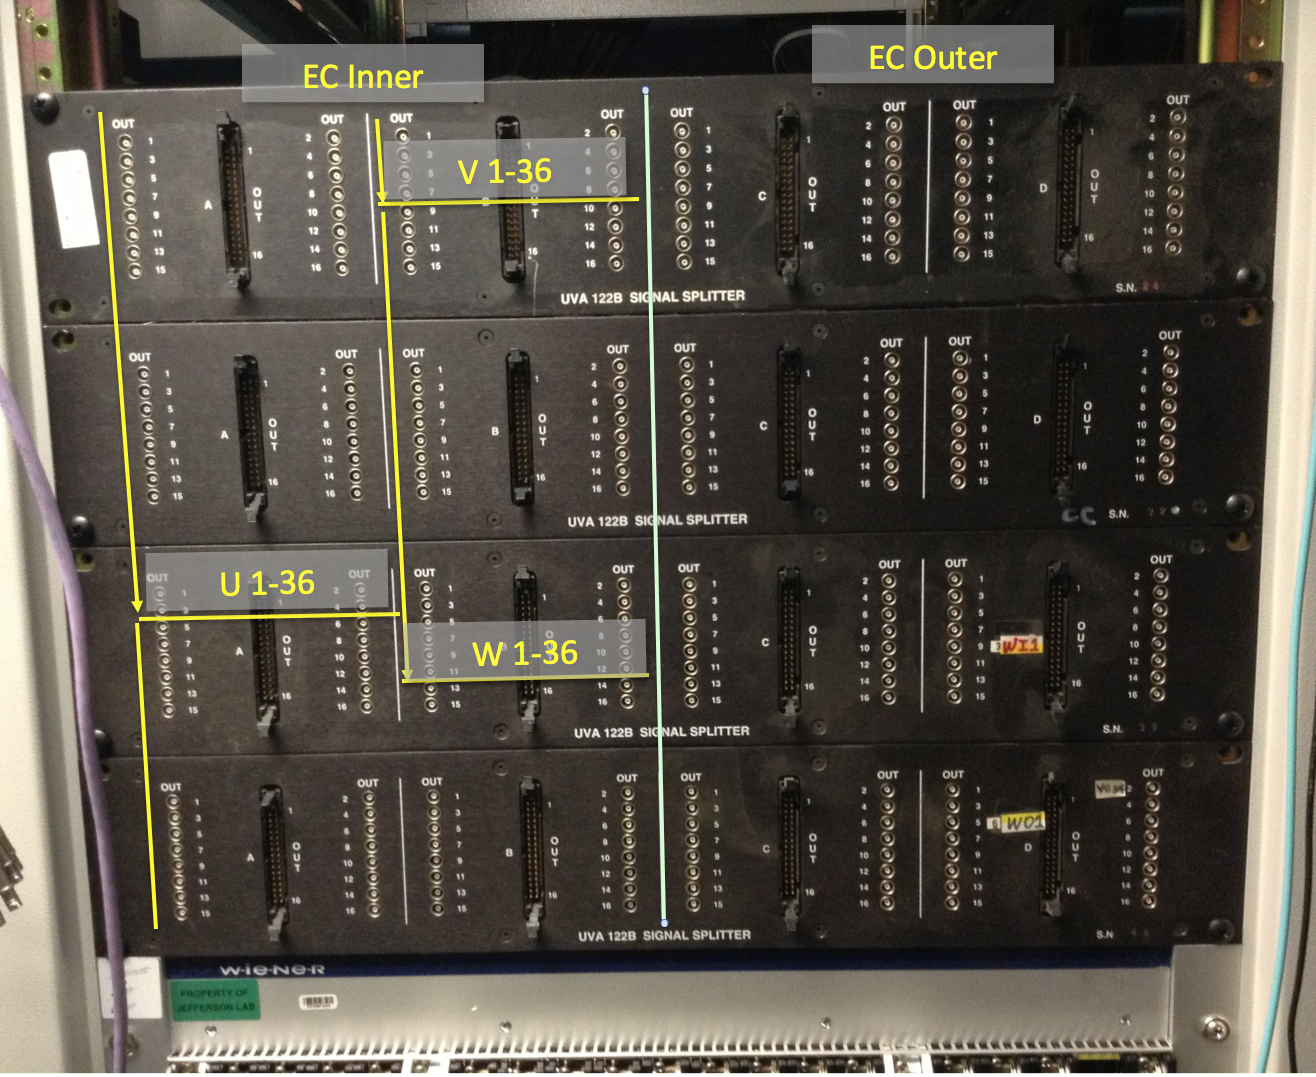
\includegraphics[width= 7in, keepaspectratio = true]{ecal-pp-2.png}
\caption{Photo of ECAL UVA122B splitter panels.  LEMO inputs are in the rear.  LEMO outputs are used
  for FADC connections and the mapping used for EC Inner is illustrated with the yellow overlay.  The 17-pin connector
  is used for mini-coax connections to the DSC2 discriminators.  The split ratio is 3:1, with 3/4 going
  to the FADC and 1/4 going to the DSC2.  The EC Outer mapping is identical.}
\label{ecal-pp-2}
\end{figure}
%%%%%%%%%%%%%%%%%%%%%%%%%%%%%%%%%%%%%%%%%%%%%%%%%%%%%%%%%%%%%%%%%%%%%%%%%%%%%%%%%%%%%%%%%%%%%%%%%%%%%

\subsubsection{Altering Cable Maps}

The nominal procedure if there is a problem with a VME electronics board is to replace the board
with a spare unit.  However, for testing purposes, it might be necessary to change a signal input
at the FADC, discriminator, or TDC to an unused channel. For PCAL there are no unused channels,
while for ECAL there are a total of eight unused channels for both FADCs and DSCs.  Utilizing
unused channels for the TDCs is limited due to the use of ribbon cable.  Any remapping of channels
must be done in coordination with the DAQ system expert in order to update the database translation 
tables. This operation is not something that is normally done and should not be attempted by shift
workers or EC experts as it could lead to problems decoding the data.

Problems with channels within the HV system may arise due to connection failures at the 24 pin
interface between the HV distribution box and the A1535N board, or failures of the board itself.
The standard procedure when there is a problem with a CAEN HV board is to swap out the board
(see Section~\ref{board-swap}).  As indicated there are no spare channels in either ECAL or PCAL.
An unlikely possibility is failure of a single slot in the HV mainframe, which would require
moving a HV board to an unused slot. This would require reprogramming the EPICS Slow Controls database
to ensure smooth operation of the HV Control GUIs and should be done only in consultation with a
Slow Controls expert. 


%%%%%%%%%%%%%%%%%%%%%%%%%%%%%%%%%%%%%%%%%%%%%%%%%%%%%%%%%%%%%%%%%%%%%%%%%%%%%%%%%%%%%%%%%%%%%%%%%%%%%
\begin{sidewaysfigure}[htbp]
  \hspace{1cm}
  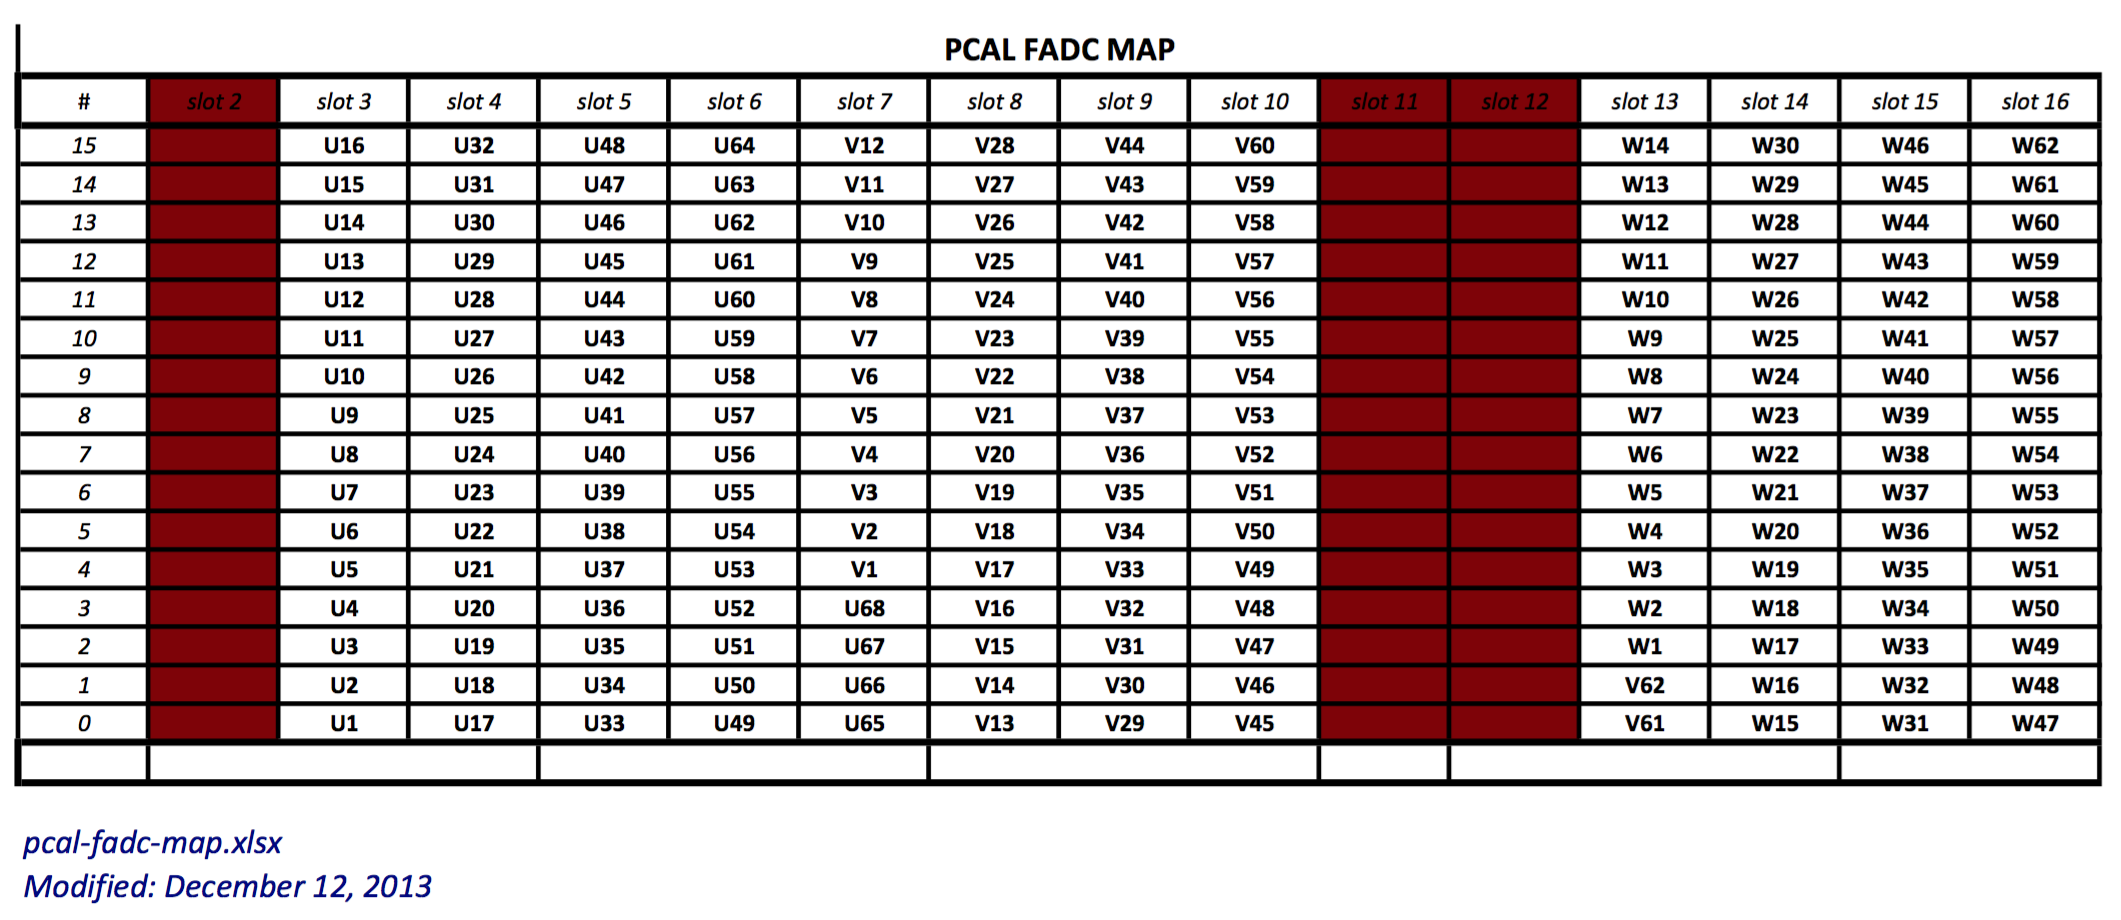
\includegraphics[width=9in]{pcal-fadc-map}
  \caption{Electronics map for the input connections to the PCAL VME FADCs.  Slots 11 and 12 are
  reserved for the Virtual Trigger Processor (VTP).}
  \label{pcal-fadc-map}
\end{sidewaysfigure}
%%%%%%%%%%%%%%%%%%%%%%%%%%%%%%%%%%%%%%%%%%%%%%%%%%%%%%%%%%%%%%%%%%%%%%%%%%%%%%%%%%%%%%%%%%%%%%%%%%%%%

%%%%%%%%%%%%%%%%%%%%%%%%%%%%%%%%%%%%%%%%%%%%%%%%%%%%%%%%%%%%%%%%%%%%%%%%%%%%%%%%%%%%%%%%%%%%%%%%%%%%%
\begin{sidewaysfigure}[htbp]
  \hspace{1cm}
  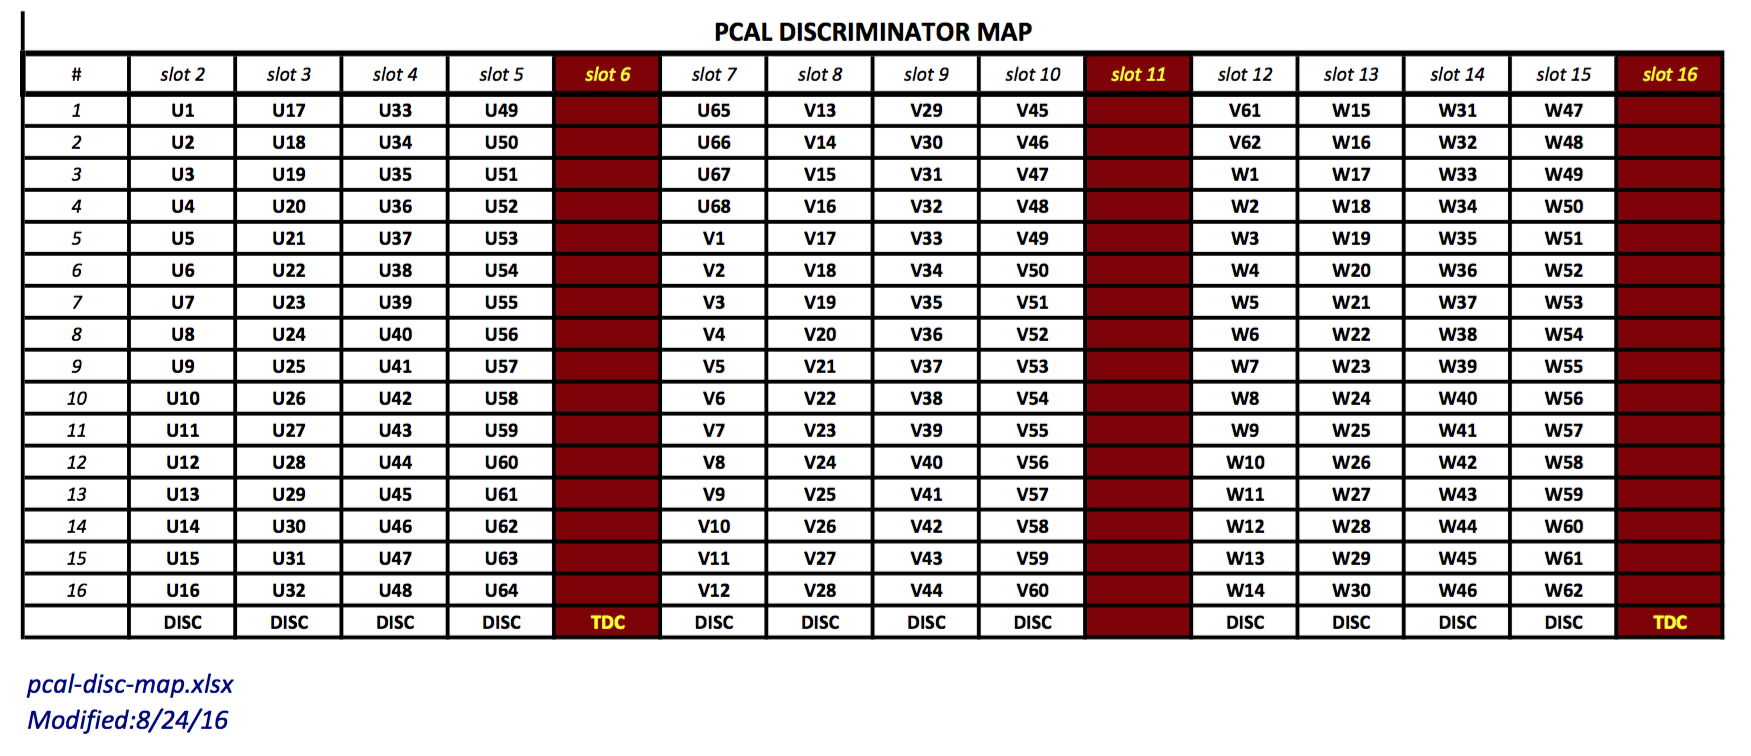
\includegraphics[width=9in]{pcal-disc-map}
  \caption{Electronics map for the input connections to the PCAL VME discriminators. Twisted-pair ribbon
  cables make the connections to the V1190 TDCs is slots 6 and 16.}
  \label{pcal-disc-map}
\end{sidewaysfigure}
%%%%%%%%%%%%%%%%%%%%%%%%%%%%%%%%%%%%%%%%%%%%%%%%%%%%%%%%%%%%%%%%%%%%%%%%%%%%%%%%%%%%%%%%%%%%%%%%%%%%%

%%%%%%%%%%%%%%%%%%%%%%%%%%%%%%%%%%%%%%%%%%%%%%%%%%%%%%%%%%%%%%%%%%%%%%%%%%%%%%%%%%%%%%%%%%%%%%%%%%%%%
\begin{sidewaysfigure}[htbp]
  \hspace{1cm}
  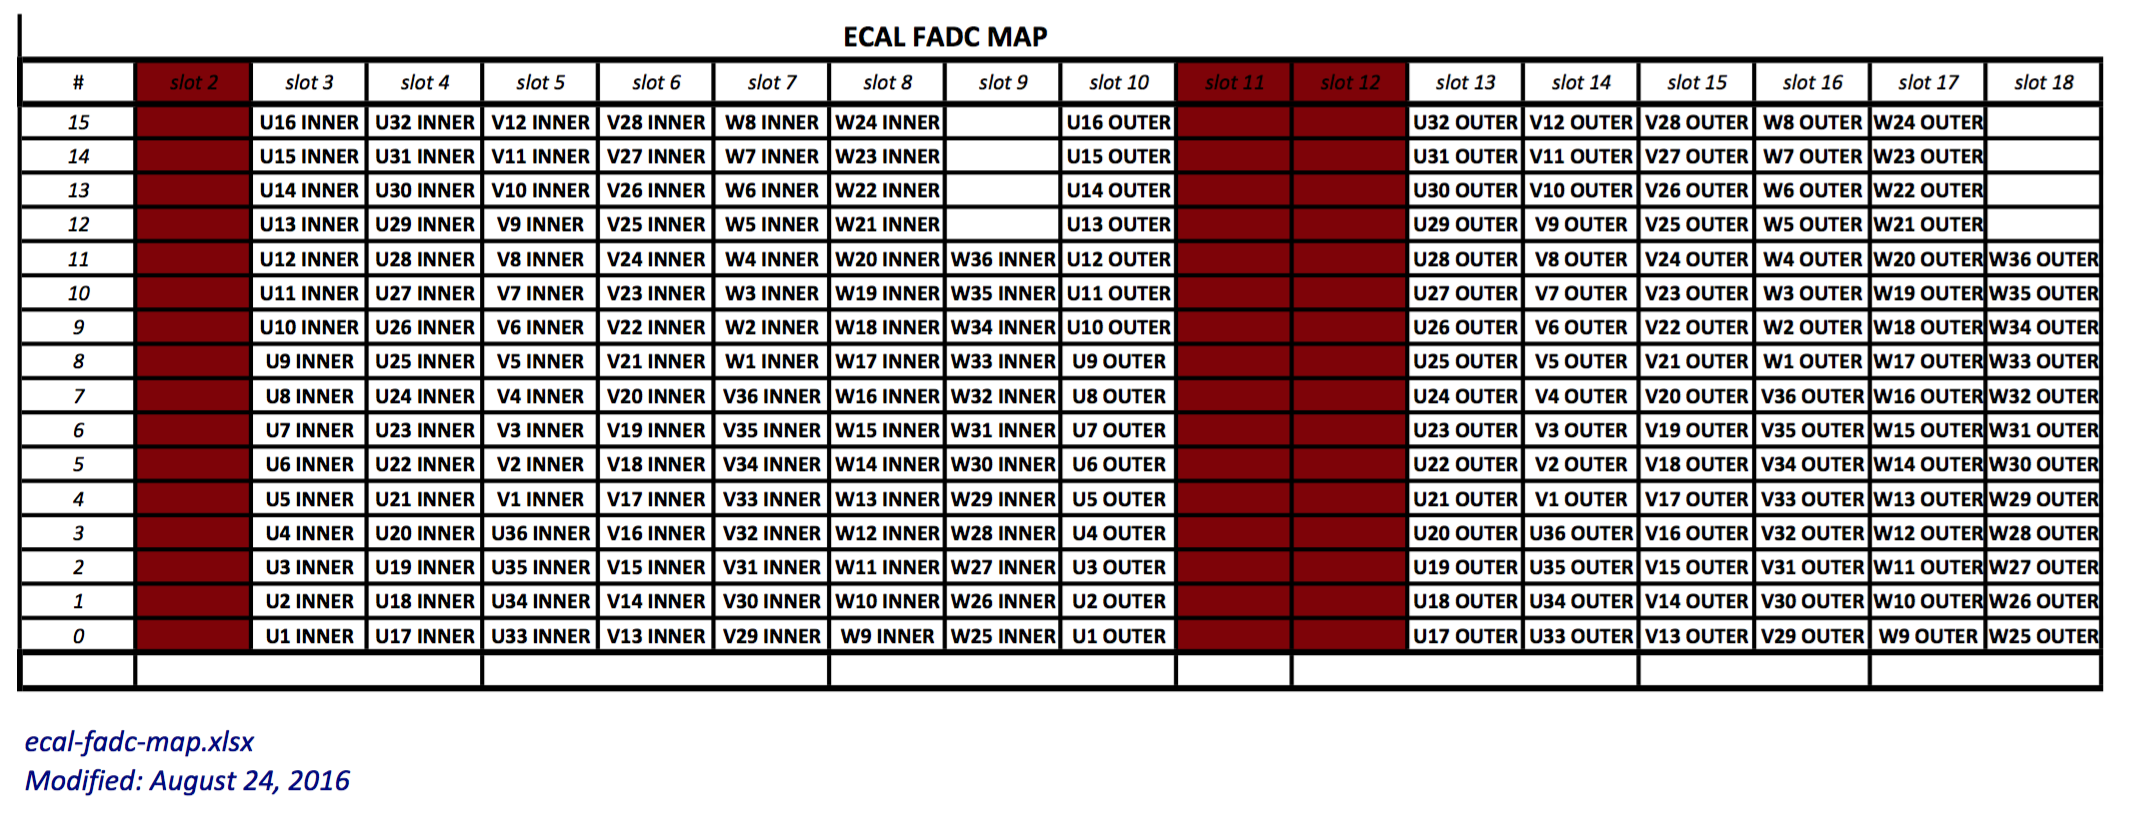
\includegraphics[width=9in]{ecal-fadc-map}
  \caption{Electronics map for the input connections to the ECAL VME FADCs. Slots 11 and 12 are
  reserved for the Virtual Trigger Processor (VTP).}
  \label{ecal-fadc-map}
\end{sidewaysfigure}
%%%%%%%%%%%%%%%%%%%%%%%%%%%%%%%%%%%%%%%%%%%%%%%%%%%%%%%%%%%%%%%%%%%%%%%%%%%%%%%%%%%%%%%%%%%%%%%%%%%%%

%%%%%%%%%%%%%%%%%%%%%%%%%%%%%%%%%%%%%%%%%%%%%%%%%%%%%%%%%%%%%%%%%%%%%%%%%%%%%%%%%%%%%%%%%%%%%%%%%%%%%
\begin{sidewaysfigure}[htbp]
  \hspace{1cm}
  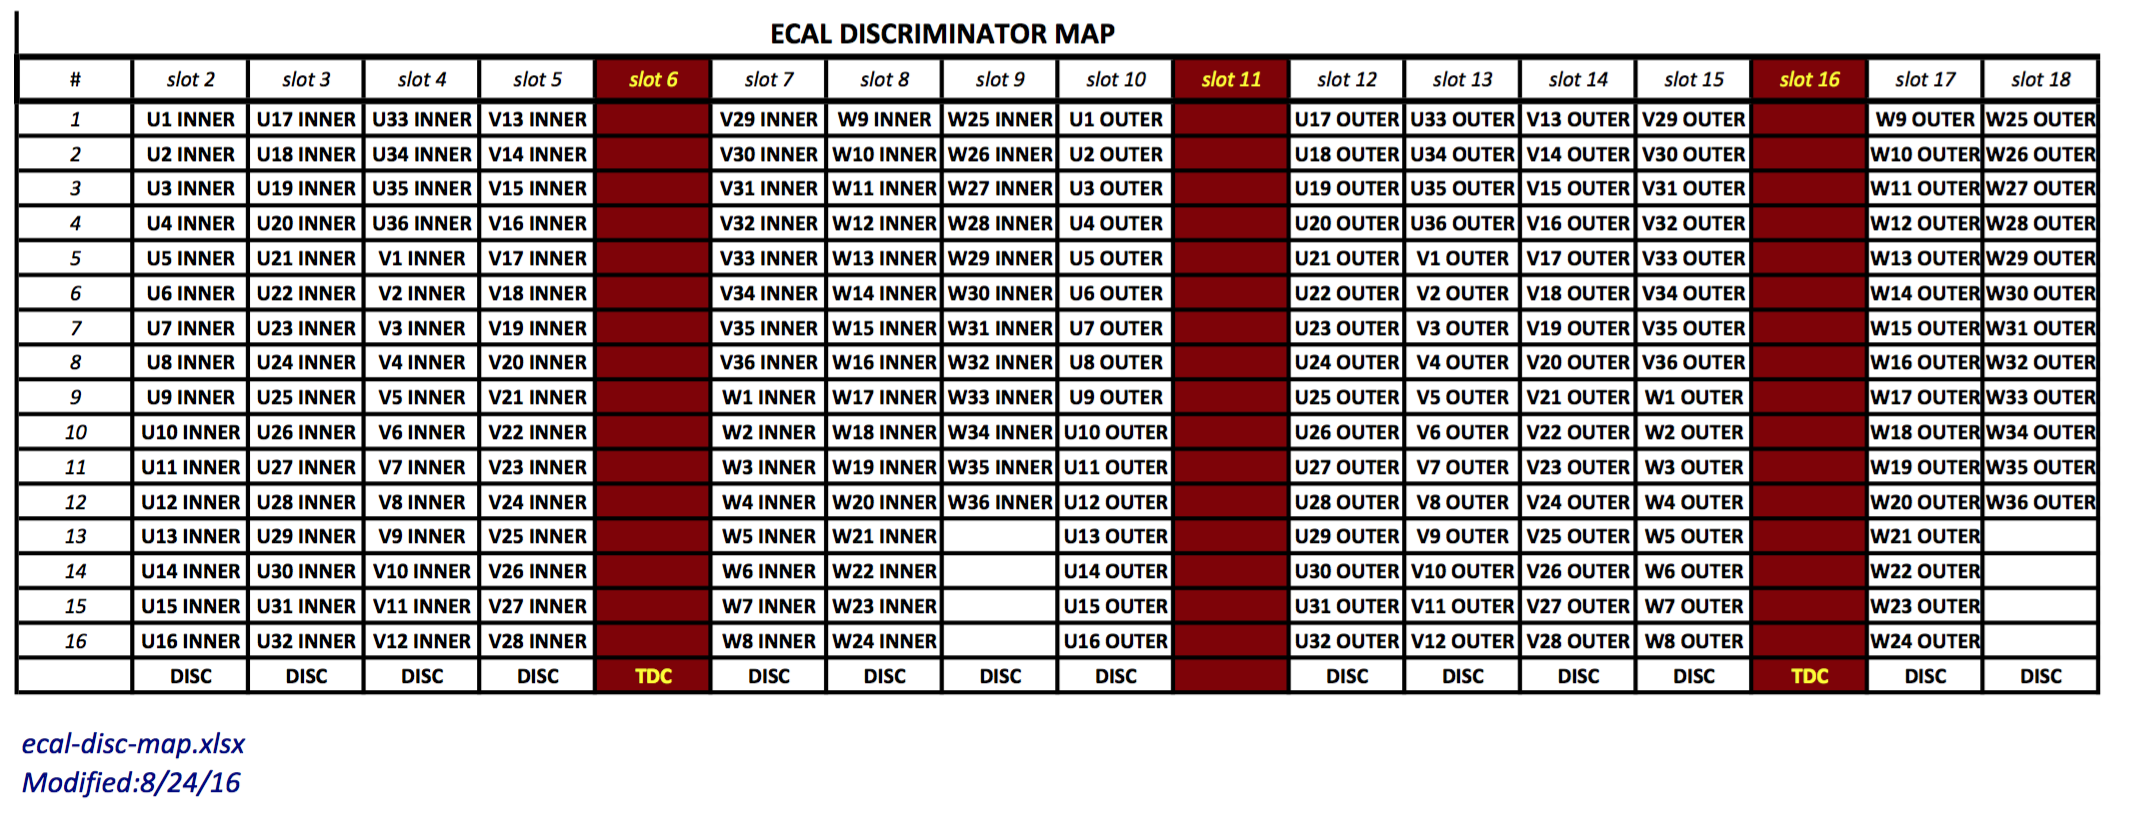
\includegraphics[width=9in]{ecal-disc-map}
  \caption{Electronics map for the input connections to the ECAL VME discriminators.  Twisted-pair ribbon
  cables make the connections to the V1190 TDCs is slots 6 and 16.}
  \label{ecal-disc-map}
\end{sidewaysfigure}
%%%%%%%%%%%%%%%%%%%%%%%%%%%%%%%%%%%%%%%%%%%%%%%%%%%%%%%%%%%%%%%%%%%%%%%%%%%%%%%%%%%%%%%%%%%%%%%%%%%%%


%%%%%%%%%%%%%%%%%%%%%%%%%%%%%%%%%%%%%%%%%%%%%%%%%%%%%%%%%%%%%%%%%%%%%%%%%%%%%%%%%%%%%%%%%%%%%%%%%%%%%
\begin{sidewaysfigure}[htbp]
  \hspace{1cm}  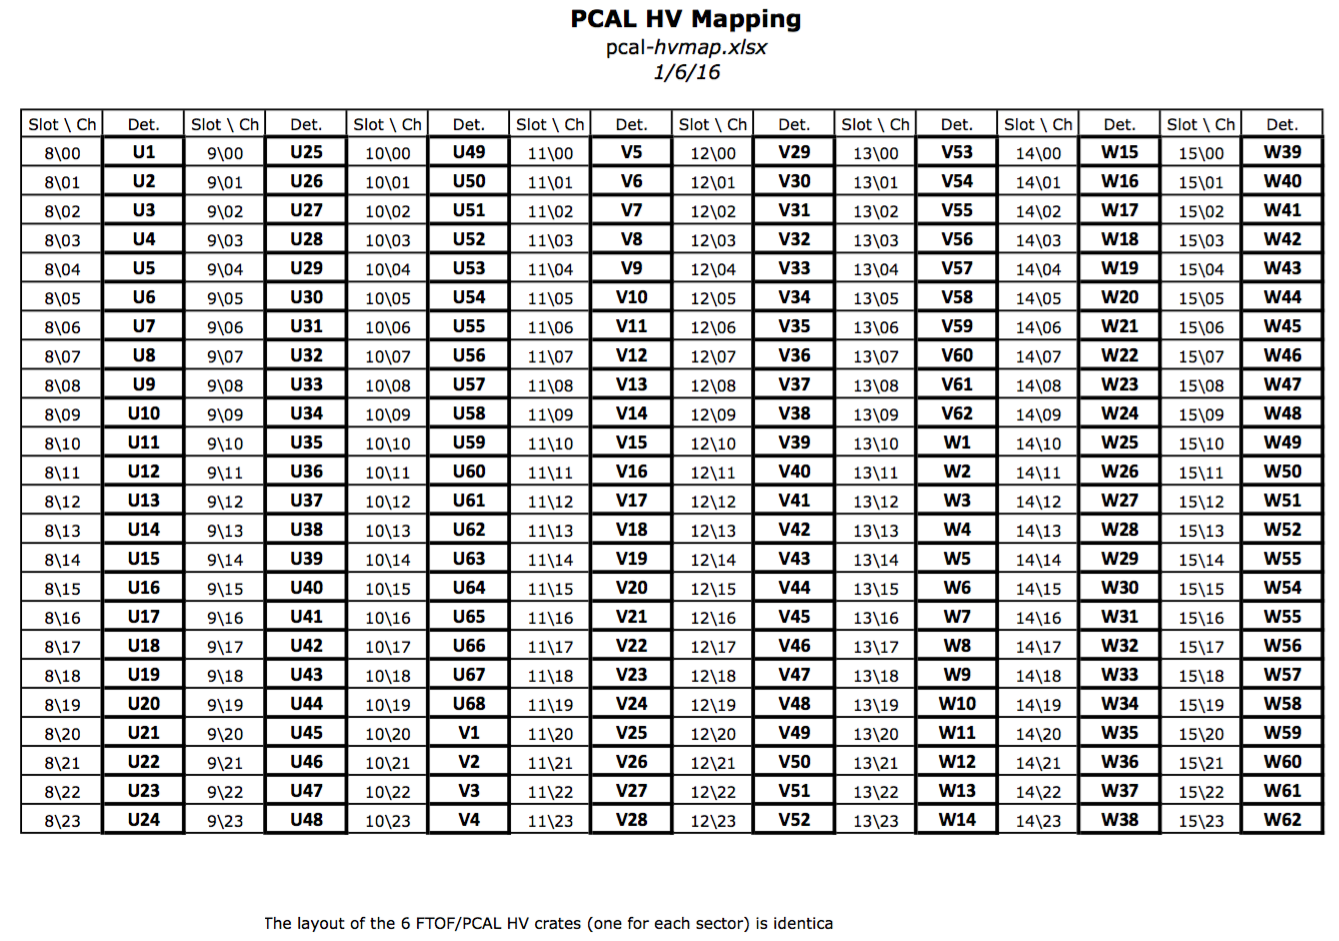
\includegraphics[width=9in]{pcal-hv-map}
\caption{HV mainframe PCAL channel assignments for each sector.}
\label{pcal-hv-map}
\end{sidewaysfigure}
%%%%%%%%%%%%%%%%%%%%%%%%%%%%%%%%%%%%%%%%%%%%%%%%%%%%%%%%%%%%%%%%%%%%%%%%%%%%%%%%%%%%%%%%%%%%%%%%%%%%%
%%%%%%%%%%%%%%%%%%%%%%%%%%%%%%%%%%%%%%%%%%%%%%%%%%%%%%%%%%%%%%%%%%%%%%%%%%%%%%%%%%%%%%%%%%%%%%%%%%%%%
\begin{sidewaysfigure}[htbp]
  \hspace{1cm}
  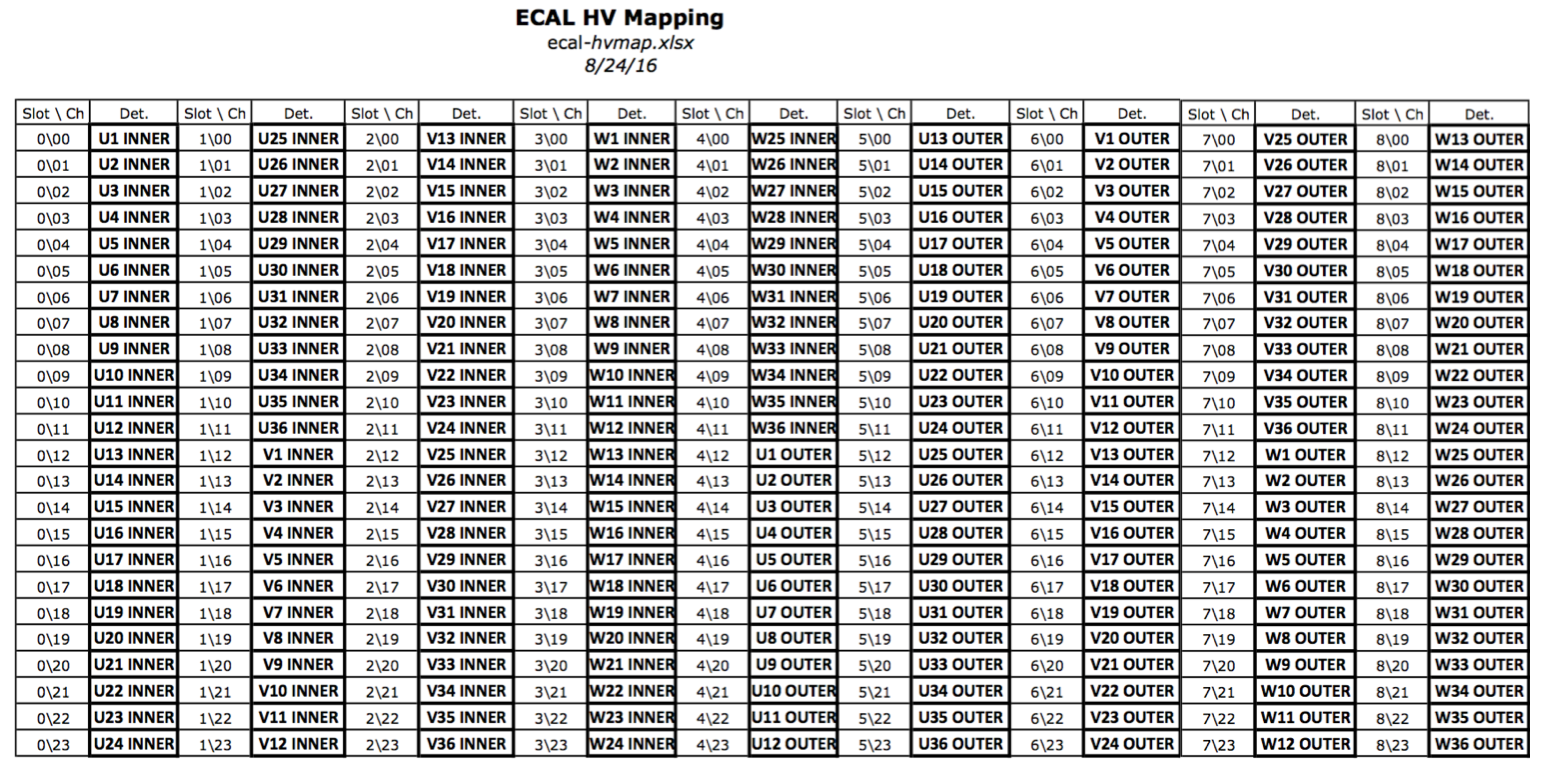
\includegraphics[width=9in]{ecal-hv-map}
\caption{HV mainframe ECAL channel assignments for each sector.}
\label{ecal-hv-map}
\end{sidewaysfigure}
%%%%%%%%%%%%%%%%%%%%%%%%%%%%%%%%%%%%%%%%%%%%%%%%%%%%%%%%%%%%%%%%%%%%%%%%%%%%%%%%%%%%%%%%%%%%%%%%%%%%%

\newpage

\subsection{System Failure Modes}
\label{repairs}

For the EC detector, there are a number of usual ``failure'' modes with which the system expert should
be familiar. These include the following:

\begin{itemize}
\item Replacing a HV board (see Section~\ref{board-swap}).
\item Sudden ADC gain shift (see Section~\ref{gain-shift}).
\item High PMT dark current (see Section~\ref{high-current}).
\item Missing anode signal (see Section~\ref{missing}).
\item Bad PMT (see Section~\ref{bad-pmt}).
\item Readout electronics issues (see Section~\ref{readout-issues}).
\item IOC issues (see Section~\ref{ioc-issues}).
\end{itemize}

\subsubsection{HV Board Replacement}
\label{board-swap}

The evidence for a bad HV board (A1535N) is either that the 24 channels associated with a single 
board won't ramp up to full voltage before tripping off or bad voltage regulation. For the case
of bad voltage regulation, the channels ramp up to full voltage but then fluctuate about the demand 
voltage setting by up to several hundred volts. Before deciding whether a HV board is bad, some
investigation should be completed to ensure that a single HV channel is not causing the problems
with the board, which could point to a problem with the PMT or voltage divider. If a board is deemed 
bad and needs to be replaced, the following steps are necessary:

\begin{enumerate}
\item Take a spare A1535N board from the storage area on the second level of the Pie Tower in Hall~B.
\item Turn the front panel key on the HV supply to the ``off'' position and toggle the main power 
switch to ``off'' on the back of the HV supply.
\item On the back of the supply, remove the Radiall connector on the bad board.
\item Pull out the bad board, being careful of the Radiall connectors on the neighboring boards.
\item Install the new board and reconnect the Radiall connector.
\item Toggle the main power switch to ``on'' and turn the HV power supply on using the key on the front 
panel, putting the key in the ``local'' position.
\item Run all parameter scripts for the HV power supply to load all channel parameters. See instructions
in Section~\ref{hv-parms}.
\item Enter information on the new board and the old bad board into the Hall~B equipment database (see
the Appendix).
\item Leave the bad board on the RadCon Survey table in Hall~B.
\end{enumerate}

\subsubsection{Sudden Gain Shift}
\label{gain-shift}

Sometimes a sudden gain shift can appear in the ADC spectra for a given counter. There are a number of
possible causes for such a condition.

\begin{itemize}
\item Problematic PMT - sometimes gain shifts can be attributed to a problem with a PMT that requires 
adjustment of the HV settings. Of course, PMT gain issues typically lead to a reduced gain that requires 
an increase of the HV. 
\item DAQ Problems - the most common cause for an apparent gain shift in the ADC spectra for a counter is 
due to problems with the FADC settings. Such problems can typically be diagnosed from pedestal shifts or 
widened pedestals. The pedestals can be checked by taking FADC data in ``raw mode''.
\item Light Leak - it is possible that a gain shift can be due to hardware damage or a light leak on the 
counter.
\end{itemize}

\subsubsection{High PMT Dark Current}
\label{high-current}

\subsubsection{Missing Anode or Dynode Signal}
\label{missing}


\subsubsection{Bad PMT}
\label{bad-pmt}

One of the most common failure modes of a PMT is a gradual loss of gain over the period of
several years. This can be compensated by adjusting the HV to maintain the gain setting. The
PMTs used in the EC system have maximum voltage ratings of -2500~V for the ECAL PMTs and
-1100~V for the PCAL PMTs.  Once the PMT HV is set to its maximum value
and the gain falls below the nominal setting, the PMT should be flagged for replacement during
the next servicing opportunity.

\subsubsection{Readout Electronics Issues}
\label{readout-issues}

Readout electronics issues, typically associated with all channels associated with a given
discriminator board, TDC board, or FADC board, once diagnosed should be brought to the
attention of the DAQ system expert for further diagnosis and attention.

\subsubsection{IOC Issues}
\label{ioc-issues}

Loss of communication between the IOC and the HV mainframe is seen by a yellow color status for
all HV channels in a given sector. The IOC should be reset following the instructions given in
Section~\ref{hv-control}. If resetting the IOC does not solve the problems, contact the 
Slow Controls system expert.

\subsection{Detector Repairs and Servicing}

Repairs and servicing of the physical structure of the EC detectors is limited to maintaining
light-tight tape seals along the known openings and sheet metal seams.  Black 3M tape is visible
in numerous locations and usually indicates where energized PMTs were able to detect significant
light leaks.  These seals must be maintained to prevent excessive count rates in the PMTs.  Repair
and replacement of defective PMTs and HV dividers will be necessary as time passes. 

All EC detector repairs will be organized through the EC Group Leader in conjunction with the
Hall~B Work Coordinator to be scheduled during a planned major down time for Hall~B.

\clearpage

\vfil
\eject

\section{Documentation}

All current documentation for the EC system is located on the official EC web page~\cite{ecal-web}. 
A number of basic subsystem documents can be found there including:

\begin{itemize}
\item EC System Operations Manual (this document)
\item EC Geometry Document
\item EC Calibration Constants
\item EC Monte Carlo Simulation Details
\item EC Reconstruction Document
\item Assorted photographs of the detector hardware
\end{itemize}

\section{EC Authorized Personnel}
\label{personnel}

Beyond turning on/off the EC system HV and monitoring the system scalers, all other operations and
repairs are only to be carried out by the list of authorized personnel shown in Table~\ref{expert-list}.
The list of authorized personnel for EC can only be modified by the EC Group Leader.

%%%%%%%%%%%%%%%%%%%%%%%%%%%%%%%%%%%%%%%%%%%%%%%%%%%%%%%%%%%%%%%%%%%%%%%%%%%%%%%%%%%%%%%%%%%%%%%%%%%%%
\begin{table}[htbp]
\begin{center}
\begin{tabular} {|c|c|c|c|} \hline
Name             & Telephone    & email              & Area             \\ \hline \hline
Stepan Stepanyan & 757-269-7196 & stepanya@jlab.org  & EC Group Leader  \\ \hline
Cole Smith       & 434-249-4307 & lcsmith@jlab.org   & Hardware         \\ \hline
Daniel Carman    & 757-269-5586 & carman@jlab.org    & Hardware         \\ \hline
Sergey Boyarinov & 757-269-5795 & boyarinov@jlab.org & DAQ              \\ \hline
Nathan Baltzell  & 757-269-5902 & baltzell@jlab.org  & Slow Controls    \\ \hline
\end{tabular}
\caption{EC detector authorized personnel.}
\label{expert-list}
\end{center}
\end{table}
%%%%%%%%%%%%%%%%%%%%%%%%%%%%%%%%%%%%%%%%%%%%%%%%%%%%%%%%%%%%%%%%%%%%%%%%%%%%%%%%%%%%%%%%%%%%%%%%%%%%%

\clearpage

\vfil
\eject

\section{Appendix: Hall~B Instrumentation Database}

When electronics modules or HV modules are removed from Hall~B and replaced during servicing with
new boards, the information regarding both the old board and the new board need to be entered into
the Hall~B Instrumentation Database. This database is accessed online at http://clonwiki0.jlab.org
by clicking on the ``Hall~B Inventory'' link. This brings up the access screen shown in 
Fig.~\ref{inventory}. To enter information for the old component, search for it in the database using
its property tag information. When the item shows up, click on the ``Action'' button for
``Modify this item''. Be sure to change the location of the item to ``Hall~B Underground/RadCon Table''
and change the status of the item to ``Action needed/Broken'', as well as to leave the item on the
RadCon survey table in Hall~B. By entering this information, email will be sent to the property custodian
to pick up the item for servicing. For the new component, be sure to also change the location as
appropriate using the same approach.

%%%%%%%%%%%%%%%%%%%%%%%%%%%%%%%%%%%%%%%%%%%%%%%%%%%%%%%%%%%%%%%%%%%%%%%%%%%%%%%%%%%%%%%%%%%%%%%%%%%%%
\begin{figure}[htbp]
  \centering
  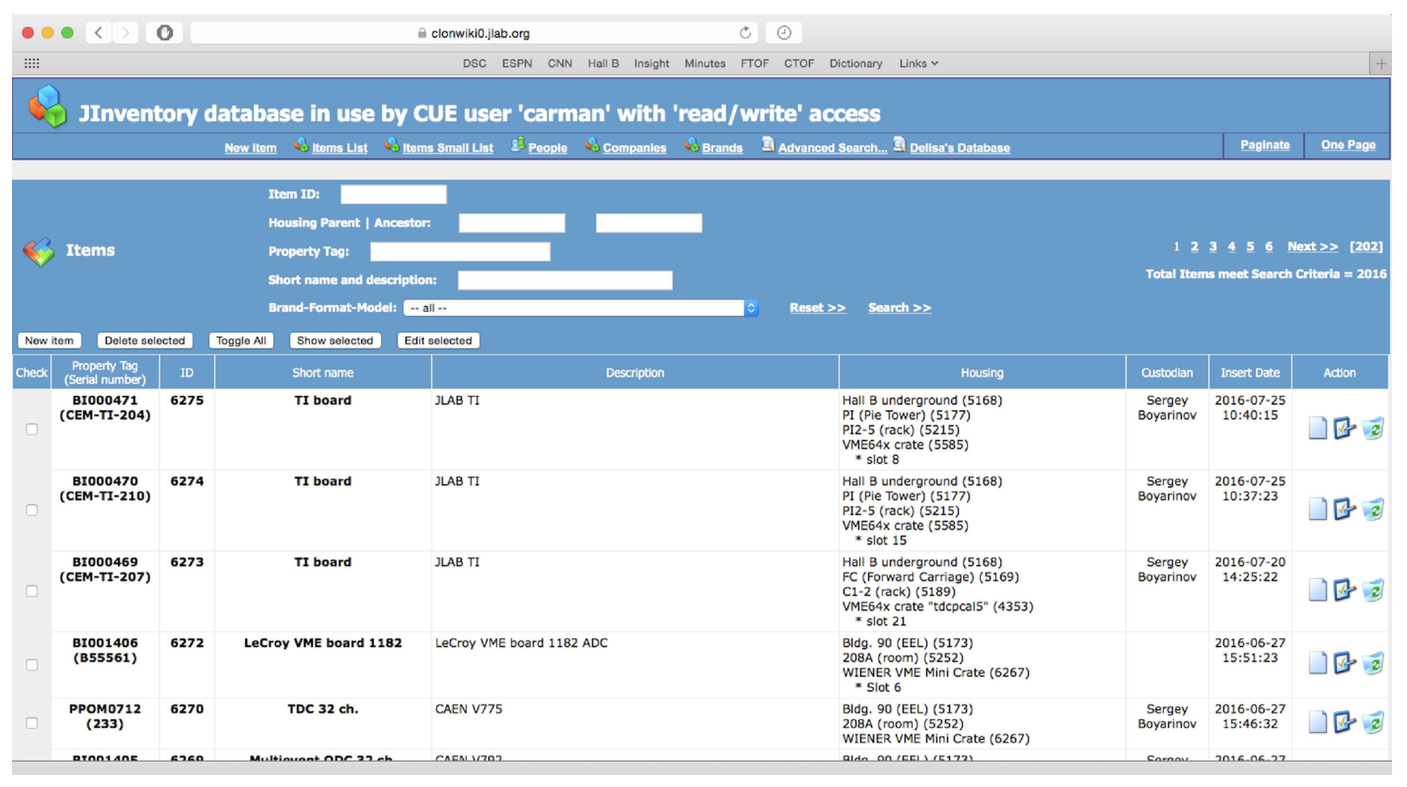
\includegraphics[width= 7in, keepaspectratio = true]{inventory}
  \vspace{2mm}
\caption{Hall~B equipment database web page.}
\label{inventory}
\end{figure}
%%%%%%%%%%%%%%%%%%%%%%%%%%%%%%%%%%%%%%%%%%%%%%%%%%%%%%%%%%%%%%%%%%%%%%%%%%%%%%%%%%%%%%%%%%%%%%%%%%%%%

\clearpage

\vfil
\eject

\begin{thebibliography}{99}

\bibitem{e-log}
  Hall~B Electronic Logbook: https://logbooks.jlab.org/book/hblog

\bibitem{beast}
  Hall~B BEAST alarm handler: \\
  https://clasweb.jlab.org/wiki/index.php/Slow\_Control\_Alarms

\bibitem{fcmon}
  FCMON:\\
  https://github.com/forcar/fc/wiki/FCMON  

\bibitem{ecal-web}
  EC web page: \\
  https://clasweb.jlab.org/wiki/index.php/CLAS12\_Forward\_Electromagnetic\_Calorimeter
  
\end{thebibliography}





\end{document}
